% =============================================================================
% main.tex  |  Slides do workshop "Técnicas de Avaliação de Políticas Públicas"
% Compilar (a partir da pasta slides/):  pdflatex main.tex  (2x)   ou   latexmk -pdf main.tex
% As figuras vêm de ../figuras (geradas pelos scripts R: ver README).
% =============================================================================
\documentclass[aspectratio=169,11pt,table]{beamer}
% =============================================================================
% 00_preambulo.tex  |  Tema e macros dos slides
% Workshop: Técnicas de Avaliação de Políticas Públicas (EACH/USP, 2026)
% Paleta inspirada no cartaz do Seminário Discente 2026 (laranja + índigo).
% =============================================================================
\usepackage[utf8]{inputenc}
\usepackage[T1]{fontenc}
\usepackage[brazil]{babel}
\usepackage{lmodern}
\usepackage{graphicx}
\usepackage{booktabs}
\usepackage{tikz}
\usetikzlibrary{arrows.meta,positioning,shapes.geometric,calc,fit,backgrounds,decorations.pathreplacing}
\usepackage{listings}
\usepackage{xcolor}
\usepackage{tabularx}
\usepackage{array}

\graphicspath{{../figuras/}}

% ---- Cores --------------------------------------------------------------------
\definecolor{laranja}{HTML}{F26B21}
\definecolor{indigo}{HTML}{4A55A2}
\definecolor{cinza}{HTML}{8E93B0}
\definecolor{verde}{HTML}{2E8B57}
\definecolor{fundo}{HTML}{F8F8F8}
\definecolor{indigoclaro}{HTML}{E4E6F3}
\definecolor{laranjaclaro}{HTML}{FDE8DC}

% ---- Aparência geral -----------------------------------------------------------
\usetheme{default}
\usefonttheme{professionalfonts}
\renewcommand{\familydefault}{\sfdefault}
\setbeamertemplate{navigation symbols}{}
\setbeamercolor{background canvas}{bg=fundo}
\setbeamercolor{normal text}{fg=black!85}
\setbeamercolor{structure}{fg=indigo}
\setbeamercolor{frametitle}{fg=indigo,bg=fundo}
\setbeamercolor{itemize item}{fg=laranja}
\setbeamercolor{itemize subitem}{fg=indigo}
\setbeamercolor{enumerate item}{fg=laranja}
\setbeamercolor{block title}{bg=indigo,fg=white}
\setbeamercolor{block body}{bg=indigoclaro,fg=black!85}
\setbeamercolor{alerted text}{fg=laranja}
\setbeamerfont{block title}{series=\bfseries,size=\normalsize}
\setbeamertemplate{blocks}[rounded][shadow=false]
\setbeamertemplate{itemize item}[circle]
\setbeamertemplate{itemize subitem}[circle]
\setbeamertemplate{enumerate item}{\insertenumlabel.}
\setbeamerfont{frametitle}{series=\bfseries,size=\Large}
\setbeamerfont{caption}{size=\scriptsize}

% título do slide: alinhado à esquerda com uma barra laranja
\setbeamertemplate{frametitle}{%
  \vspace{0.3cm}
  \begin{tikzpicture}[baseline=0pt]
    \fill[laranja] (0,-0.25) rectangle (0.14,0.55);
    \node[anchor=west,text=indigo,font=\Large\bfseries,text width=0.92\paperwidth] at (0.3,0.15) {\insertframetitle};
  \end{tikzpicture}
}

% rodapé: identificação e numeração
\setbeamertemplate{footline}{%
  \hbox to \paperwidth{\hspace*{0.6cm}%
    {\tiny\color{cinza}Técnicas de Avaliação de Políticas Públicas \,$\cdot$\, PPGGP EACH/USP \,$\cdot$\, Seminário Discente 2026}%
    \hfill {\tiny\color{cinza}\insertframenumber}\hspace*{0.6cm}}%
  \vspace*{0.25cm}%
}
\setlength{\leftmargini}{1.2em}

% ---- Macros --------------------------------------------------------------------
\newcommand{\fonte}[1]{\par\vfill{\tiny\color{cinza}Fonte: #1}}
\newcommand{\destaque}[1]{{\bfseries\color{laranja}#1}}
\newcommand{\ind}[1]{{\bfseries\color{indigo}#1}}
\newcommand{\cod}[1]{\texttt{\color{indigo}#1}}

% Slide de seção (fundo índigo)
\newcommand{\secao}[3]{%   #1 = número, #2 = título, #3 = tempo/subtítulo
  {\setbeamercolor{background canvas}{bg=indigo}%
  \begin{frame}[plain,noframenumbering]
    \begin{tikzpicture}[remember picture,overlay]
      \fill[laranja] (current page.south west) rectangle ++(0.5,\paperheight);
      \node[anchor=west,text=white,font=\Huge\bfseries,text width=0.8\paperwidth,align=left]
        at ([xshift=1.5cm,yshift=0.6cm]current page.west) {#2};
      \node[anchor=west,text=laranjaclaro,font=\large,align=left]
        at ([xshift=1.5cm,yshift=-1.2cm]current page.west) {#1 \,$\cdot$\, #3};
    \end{tikzpicture}
  \end{frame}}%
}

% Caixa "Hora do R" (demonstração em R)
\newenvironment{horaR}[1]{%
  \begin{beamercolorbox}[wd=\textwidth,rounded=true,leftskip=0.4cm,rightskip=0.4cm,sep=0.25cm]{laranjabox}
  {\bfseries\color{laranja}\large $\blacktriangleright$ Hora do R \,$\cdot$\, \cod{#1}}\par\smallskip
}{%
  \end{beamercolorbox}
}
\setbeamercolor{laranjabox}{bg=laranjaclaro,fg=black!85}

% Slide de atividade: bloco laranja
\newenvironment{atividadebox}[1]{%
  \setbeamercolor{block title}{bg=laranja,fg=white}
  \setbeamercolor{block body}{bg=laranjaclaro,fg=black!85}
  \begin{block}{#1}
}{%
  \end{block}
  \setbeamercolor{block title}{bg=indigo,fg=white}
  \setbeamercolor{block body}{bg=indigoclaro,fg=black!85}
}

% Trechos de código R
\lstdefinestyle{R}{
  language=R, basicstyle=\ttfamily\scriptsize, keywordstyle=\color{indigo}\bfseries,
  commentstyle=\color{verde}\itshape, stringstyle=\color{laranja},
  backgroundcolor=\color{white}, frame=single, rulecolor=\color{indigoclaro},
  breaklines=true, showstringspaces=false, columns=fullflexible, keepspaces=true,
  literate={á}{{\'a}}1 {à}{{\`a}}1 {â}{{\^a}}1 {ã}{{\~a}}1 {é}{{\'e}}1 {ê}{{\^e}}1
           {í}{{\'i}}1 {ó}{{\'o}}1 {ô}{{\^o}}1 {õ}{{\~o}}1 {ú}{{\'u}}1 {ç}{{\c c}}1
           {Á}{{\'A}}1 {É}{{\'E}}1 {Í}{{\'I}}1 {Ó}{{\'O}}1 {Ú}{{\'U}}1 {Ç}{{\c C}}1
           {°}{{\textdegree}}1
}
\lstset{style=R}

% Estilos TikZ comuns
\tikzset{
  cx/.style={draw=indigo,fill=white,rounded corners=3pt,thick,align=center,inner sep=5pt,font=\small},
  cxl/.style={draw=laranja,fill=laranjaclaro,rounded corners=3pt,thick,align=center,inner sep=5pt,font=\small},
  cxi/.style={draw=indigo,fill=indigoclaro,rounded corners=3pt,thick,align=center,inner sep=5pt,font=\small},
  seta/.style={-{Stealth[length=2.6mm]},thick,color=indigo},
  setal/.style={-{Stealth[length=2.6mm]},thick,color=laranja},
}


\title{Técnicas de Avaliação de Políticas Públicas}
\author{Anderson Henrique}
\institute{Seminário Discente 2026 \,$\cdot$\, PPGGP EACH/USP}
\date{20 de outubro de 2026}

\begin{document}

% =============================================================================
% ABERTURA (14:00 a 14:15)
% =============================================================================
\section[Abertura]{Abertura}

\begin{frame}{Programa do dia}
  \footnotesize
  \renewcommand{\arraystretch}{1.15}
  \begin{tabularx}{\textwidth}{@{}lX@{}}
    \toprule
    \textbf{Horário} & \textbf{Bloco} \\ \midrule
    14:00 a 14:15 & Abertura: por que avaliar? \\
    14:15 a 14:35 & O problema do contrafactual \\
    14:35 a 15:05 & Experimento controlado \hfill \destaque{Exercício 1} \\
    15:05 a 15:25 & Pareamento (PSM) \\
    15:25 a 15:55 & Diferença-em-diferenças \hfill \destaque{Exercício 2} \\
    \rowcolor{laranjaclaro}
    15:55 a 16:25 & \textbf{Intervalo} \\
    16:25 a 16:45 & Regressão descontínua \\
    16:45 a 16:55 & Outras técnicas e como escolher \\
    16:55 a 17:50 & Avaliação qualitativa e métodos mistos \hfill \destaque{Exercício 3} \\
    17:50 a 18:00 & Encerramento \\ \bottomrule
  \end{tabularx}
\end{frame}

\begin{frame}{O que vamos fazer}
  \begin{itemize}
    \item Entender por que \destaque{comparar} participantes e não participantes (ou antes e depois) \destaque{engana};
    \item Conhecer as principais técnicas quase-experimentais e o que cada uma assume;
    \item \ind{Simular em R}: sabemos a \emph{verdade} do programa e testamos se a técnica a recupera;
    \item Ver o que a avaliação \ind{qualitativa} e os \ind{métodos mistos} acrescentam aos números.
  \end{itemize}
  \vspace{0.3cm}
  \begin{block}{Como funciona}
    \small Aula expositiva + scripts em R comentados (demonstração) + 3 exercícios curtos.
  \end{block}
\end{frame}

\begin{frame}{Para começar: o programa funciona?}
  \begin{exerciciobox}{Enquete rápida (chat)}
    \small
    Um programa de \textbf{qualificação profissional} foi oferecido a trabalhadores que se inscreveram voluntariamente. Um ano depois, quem participou ganha, em média, \destaque{R\$ 587 a mais} por mês do que quem não participou.
  \end{exerciciobox}
  \vspace{0.2cm}
  O programa aumentou a renda dos participantes em R\$ 587?
  \begin{itemize}
    \item[(a)] Sim, o efeito é de R\$ 587
    \item[(b)] O efeito é menor que isso
    \item[(c)] Não dá para saber só com essa informação
  \end{itemize}
\end{frame}

\begin{frame}{A avaliação no ciclo de políticas públicas}
  \centering
  \begin{tikzpicture}[scale=0.85,every node/.style={transform shape}]
    \tikzset{est/.style={minimum width=2.6cm,minimum height=0.9cm,font=\footnotesize\bfseries}}
    \node[cxi,est] (n0) at (90:1.9cm and 1.9cm)    {Formação da\\agenda};
    \node[cxi,est] (n1) at (18:4.0cm and 1.9cm)    {Formulação};
    \node[cxi,est] (n2) at (-54:3.0cm and 1.9cm)   {Tomada de\\decisão};
    \node[cxi,est] (n3) at (-126:3.0cm and 1.9cm)  {Implementação};
    \node[cxl,est] (n4) at (162:4.0cm and 1.9cm)   {Avaliação};
    \foreach \a/\b in {0/1,1/2,2/3,3/4} { \draw[seta] (n\a) to[bend left=15] (n\b); }
    \draw[setal] (n4) to[bend left=15] (n0);
  \end{tikzpicture}
  \vspace{0.2cm}\par
  \small A avaliação \destaque{renova o ciclo}: informa se a política deve ser mantida, reformulada ou interrompida (políticas baseadas em evidências).
\end{frame}

\begin{frame}{Tipos de avaliação}
  \footnotesize
  \renewcommand{\arraystretch}{1.25}
  \begin{tabularx}{\textwidth}{@{}p{1.9cm}XX@{}}
    \toprule
    & \textbf{Pergunta} & \textbf{No programa Qualifica} \\ \midrule
    \ind{Processo} & As atividades aconteceram e os serviços chegaram ao público-alvo? & Quantos se inscreveram? Os cursos ocorreram? \\
    \ind{Resultados} & A situação do público-alvo mudou? & A renda dos participantes aumentou entre antes e depois? \\
    \rowcolor{laranjaclaro}
    \destaque{Impacto} & A mudança \textbf{é causada} pelo programa? & Quanto da variação de renda existe \emph{por causa} do treinamento? \\ \bottomrule
  \end{tabularx}
  \vspace{0.3cm}

  \small Também se classificam por \textbf{tempo} (\emph{ex-ante} e \emph{ex-post}) e por \textbf{quem avalia} (interna, externa, participativa).
\end{frame}

\begin{frame}{Cadeia de resultados (teoria do programa)}
  \centering
  \begin{tikzpicture}[scale=0.82,every node/.style={transform shape}]
    \foreach \i/\t/\ex/\sty in {0/Insumos/{Orçamento,\\instrutores}/cxi,1/Atividades/{Cursos de\\qualificação}/cxi,2/Produtos/{Trabalhadores\\treinados}/cxi,3/Resultados/{Uso das\\competências}/cxl,4/{Resultados\\finais}/{Renda e\\emprego}/cxl} {
      \node[\sty,minimum width=2.1cm,minimum height=0.9cm,font=\footnotesize\bfseries] (b\i) at (2.5*\i,0) {\t};
      \node[align=center,font=\scriptsize,text=azul] at (2.5*\i,-1.3) {\ex};
    }
    \foreach \i/\j in {0/1,1/2,2/3,3/4} { \draw[seta] (b\i) -- (b\j); }
    \draw[decorate,decoration={brace,amplitude=4pt,mirror},thick,azul] (-1,-2.1) -- (6,-2.1) node[midway,below=4pt,font=\footnotesize] {Implementação (sob controle do gestor)};
    \draw[decorate,decoration={brace,amplitude=4pt,mirror},thick,laranja] (6.2,-2.1) -- (11,-2.1) node[midway,below=4pt,font=\footnotesize] {Resultados (contexto e beneficiários)};
  \end{tikzpicture}
  \vspace{0.2cm}\par
  \small Avaliar impacto exige dizer \ind{quais resultados} o programa busca e \ind{por quais canais}.
\end{frame}

% =============================================================================
% O PROBLEMA DO CONTRAFACTUAL (14:20 a 14:30)   [Script 01]
% =============================================================================
\section[Contrafactual]{O problema do contrafactual}
\subsection{O problema}

\begin{frame}{O problema fundamental da inferência causal}
  Para cada pessoa só observamos \destaque{um} dos dois mundos:
  \vspace{0.2cm}
  \begin{center}
  \footnotesize
  \renewcommand{\arraystretch}{1.25}
  \begin{tabular}{lcccc}
    \toprule
    & \textbf{Participou?} & \textbf{Com programa} & \textbf{Sem programa} & \textbf{Efeito} \\ \midrule
    Ana   & sim & R\$ 2.400 & \destaque{?} & \destaque{?} \\
    Bruno & não & \destaque{?} & R\$ 2.000 & \destaque{?} \\
    Carla & sim & R\$ 2.700 & \destaque{?} & \destaque{?} \\
    Davi  & não & \destaque{?} & R\$ 1.800 & \destaque{?} \\ \bottomrule
  \end{tabular}
  \end{center}
  \vspace{0.2cm}
  \small O que não observamos é o \ind{contrafactual}. Toda técnica de avaliação de impacto é uma \destaque{estratégia para estimá-lo}.
\end{frame}

\begin{frame}{O contrafactual: a comparação ideal}
  \centering
  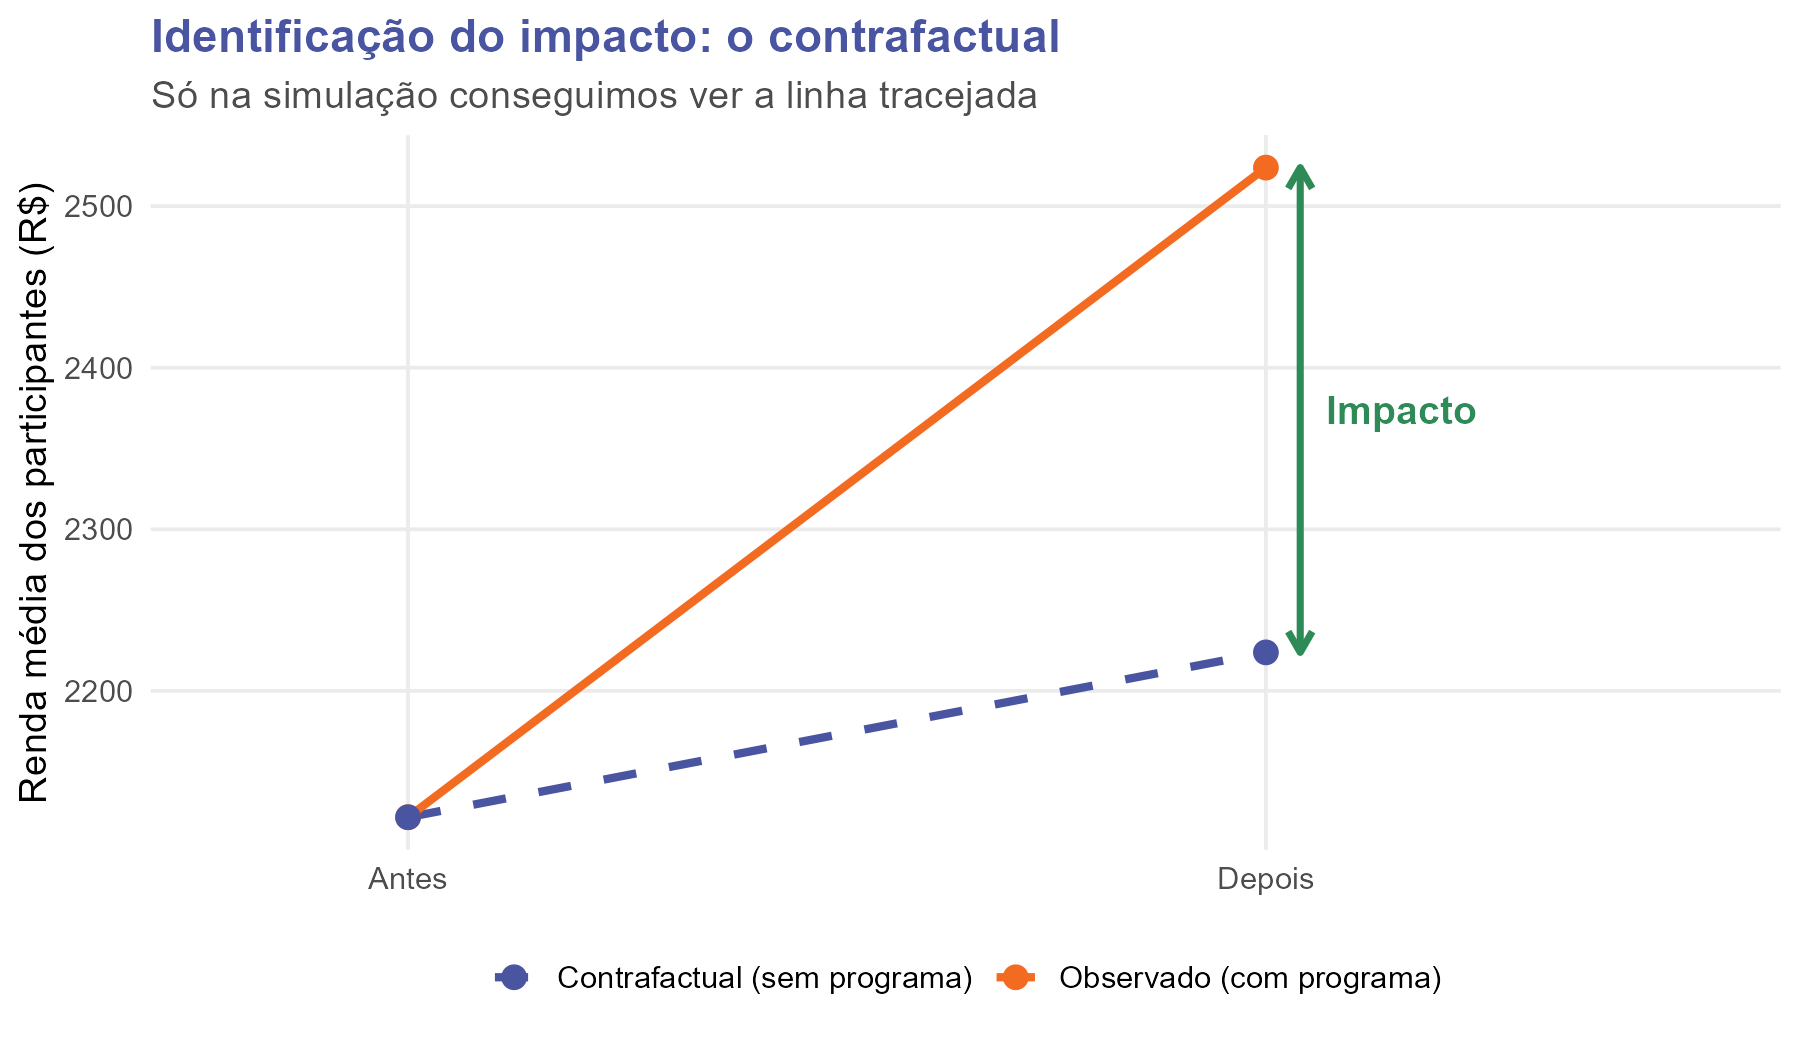
\includegraphics[height=4.6cm]{01_contrafactual.png}\par
  \footnotesize A linha tracejada nunca é observada na vida real. Só numa \ind{simulação} podemos desenhá-la.
\end{frame}

\begin{frame}{Dois falsos contrafactuais}
  \begin{columns}[T]
    \begin{column}{0.5\textwidth}
      \begin{block}{Participantes $\times$ não participantes}
        \footnotesize
        Quem participa é diferente de quem não participa (mais motivado, mais escolarizado).\\[3pt]
        \destaque{Viés de seleção.}
      \end{block}
    \end{column}
    \begin{column}{0.5\textwidth}
      \begin{block}{Antes $\times$ depois}
        \footnotesize
        A renda pode ter subido por crescimento econômico, inflação, ciclo de vida.\\[3pt]
        \destaque{Tendência no tempo.}
      \end{block}
    \end{column}
  \end{columns}
  \vspace{0.2cm}
  \centering\small Nos dois casos o efeito do programa se mistura com outros fatores.
  \vspace{0.1cm}
  \begin{block}{Voltando à enquete (dados simulados do \textit{Qualifica}, efeito verdadeiro R\$ 300)}
    \footnotesize Participantes $\times$ não: R\$ 587 (\destaque{+287}, seleção). Antes $\times$ depois: R\$ 402 (\destaque{+102}, tendência). Resposta (b): o efeito é \textbf{menor}.
  \end{block}
\end{frame}

\begin{frame}{Viés de seleção: os grupos já eram diferentes}
  \centering
  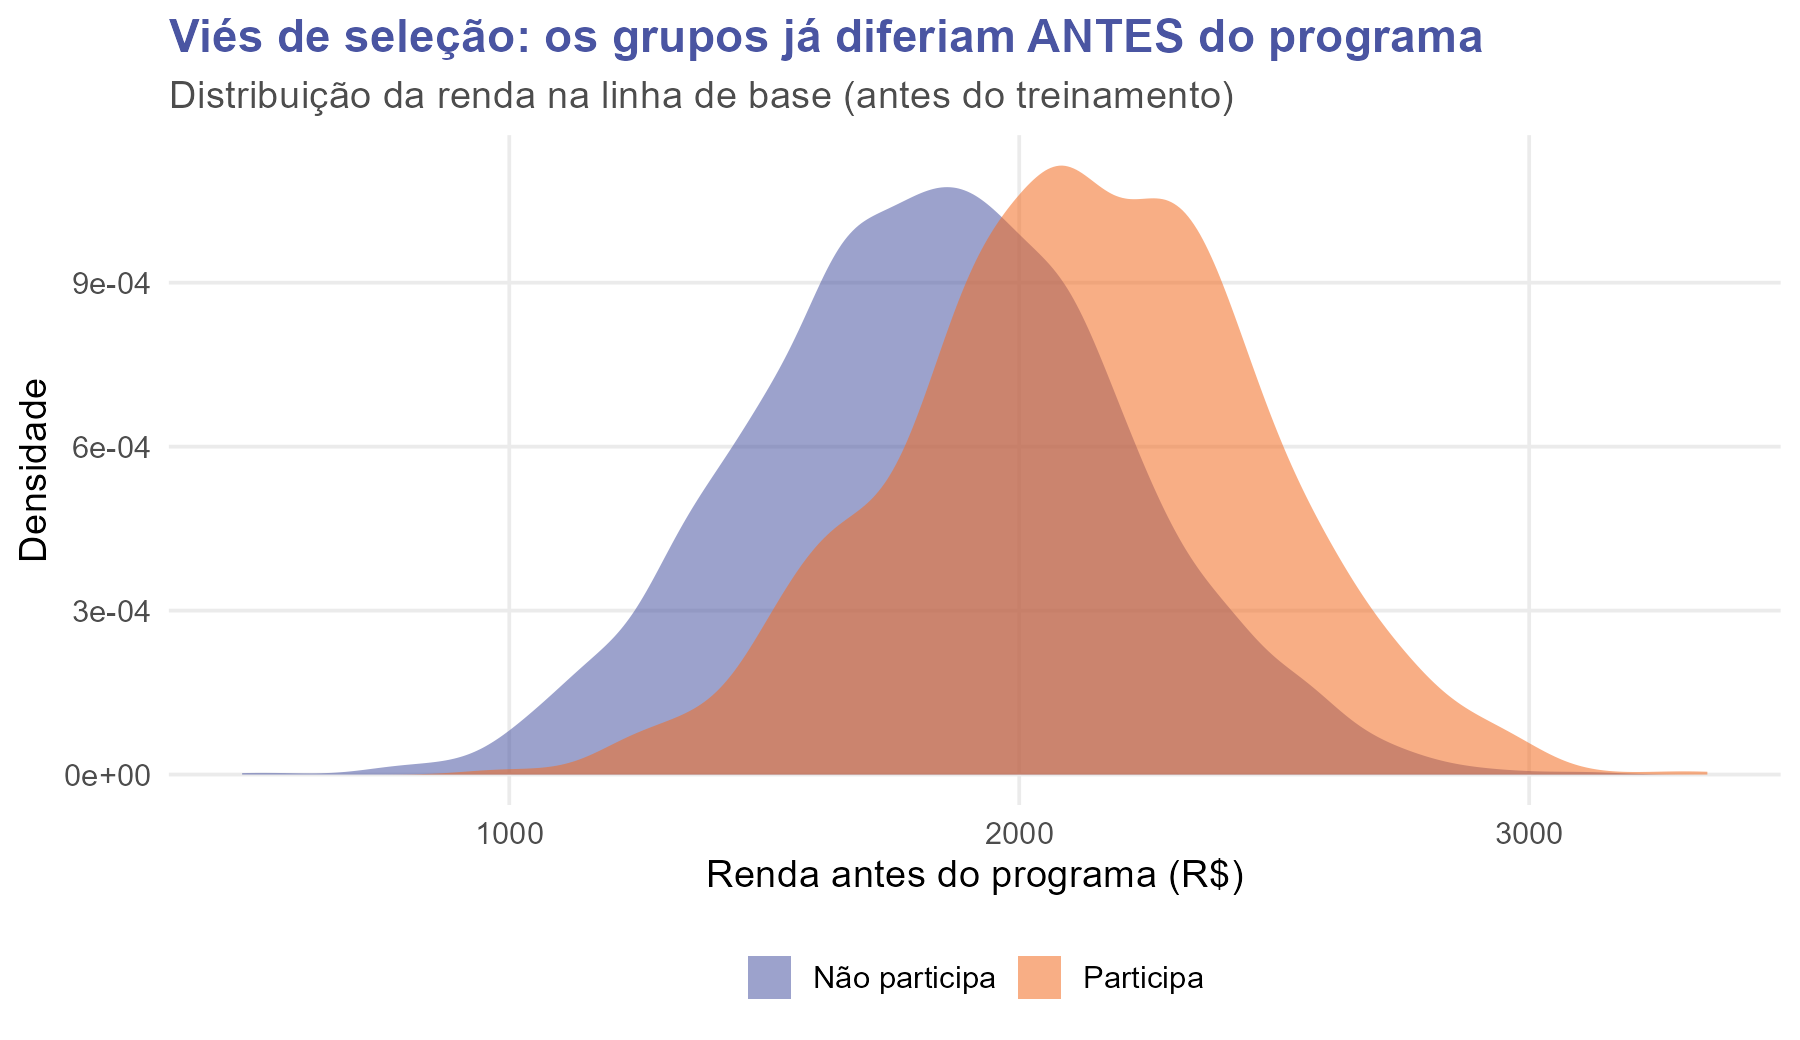
\includegraphics[height=4.2cm]{01_vies_selecao.png}\par
  \footnotesize Renda \textbf{antes} do programa: participantes R\$ 2.122; não participantes R\$ 1.836. A motivação (não observada) também difere.
\end{frame}

\subsection{Características}

\begin{frame}{Características de um bom contrafactual}
  \scriptsize
  \renewcommand{\arraystretch}{1.25}
  \begin{tabularx}{\textwidth}{@{}>{\bfseries\color{azul}\raggedright\arraybackslash}p{2.5cm}>{\raggedright\arraybackslash}X>{\raggedright\arraybackslash}X@{}}
    \toprule
    Característica & O que significa & Como checar \\ \midrule
    Comparável antes & Mesmo nível e trajetória antes da política & Balanço; pré-tendências \\
    Seleção independente & Quem entra não foi escolhido pelo que espera ganhar & Desenho (sorteio, regra) \\
    Mesmos choques & Os grupos enfrentam o mesmo contexto e período & Dados de antes e depois \\
    Sem contaminação & O controle não recebe efeitos indiretos & Distância entre unidades \\
    Mesma medida & Resultado medido igual, sem perda seletiva & Taxa de resposta por grupo \\ \bottomrule
  \end{tabularx}
  \vspace{0.2cm}\par
  \small Cada técnica garante essas características de um jeito: o \textbf{sorteio}, o \textbf{gêmeo}, a \textbf{tendência paralela}, o \textbf{corte}.
\end{frame}

\begin{frame}{Mapa das técnicas}
  \centering
  \begin{tikzpicture}[scale=0.8,every node/.style={transform shape}]
    \node[cxl,minimum width=4.2cm,minimum height=0.8cm,font=\small\bfseries] (top) at (0,0) {Identificar o impacto causal};
    \node[cxi,minimum width=3.4cm] (exp) at (-4.3,-1.7) {\textbf{Experimento}\\sorteio entre elegíveis\\(ou natural)};
    \node[cx,minimum width=3.6cm] (qe) at (1.8,-1.7) {\textbf{Quase-experimentos}\\(dados observacionais)};
    \draw[seta] (top) -- (exp); \draw[seta] (top) -- (qe);
    \node[cxi,minimum width=2.1cm] (psm) at (-1.6,-4.1) {\textbf{Pareamento}\\``gêmeos''\\observados};
    \node[cxi,minimum width=2.1cm] (did) at (1.0,-4.1) {\textbf{Dif.-em-dif.}\\tendência do\\controle};
    \node[cxi,minimum width=2.1cm] (rdd) at (3.6,-4.1) {\textbf{Reg. descont.}\\corte de\\elegibilidade};
    \node[cx,minimum width=2.1cm] (out) at (6.2,-4.1) {\textbf{Outras}\\IV, sintético,\\ponderação};
    \foreach \x in {psm,did,rdd,out} { \draw[seta] (qe) -- (\x); }
  \end{tikzpicture}
\end{frame}

% =============================================================================
% EXPERIMENTO CONTROLADO (14:25 a 14:50)   [Script 02 | Exercício 1]
% =============================================================================
\section[Experimento]{Experimento controlado}

\begin{frame}{O ``padrão ouro'': a aleatorização}
  \centering
  \begin{tikzpicture}[scale=0.8,every node/.style={transform shape}]
    \node[cx,minimum width=2.4cm] (pop) at (0,0) {Elegíveis};
    \node[cxi,minimum width=2.2cm,font=\footnotesize\bfseries] (sorteio) at (3.2,0) {Sorteio};
    \node[cxl,minimum width=2.4cm] (trat) at (6.6,1.0) {\textbf{Tratamento}};
    \node[cxi,minimum width=2.4cm] (ctrl) at (6.6,-1.0) {\textbf{Controle}};
    \node[cxl,minimum width=2.2cm,font=\footnotesize\bfseries] (imp) at (10.2,0) {Impacto\\$=\bar Y_T-\bar Y_C$};
    \draw[seta] (pop) -- (sorteio);
    \draw[seta] (sorteio) -- (trat); \draw[seta] (sorteio) -- (ctrl);
    \draw[seta] (trat) -- (imp); \draw[seta] (ctrl) -- (imp);
  \end{tikzpicture}
  \vspace{0.2cm}
  \begin{itemize}
    \item O sorteio torna os grupos equivalentes \destaque{em média}, nas características observadas e \textbf{não observadas};
    \item Só difere o receber ou não a política: a diferença nos resultados é o \ind{impacto}.
  \end{itemize}
\end{frame}

\begin{frame}{Experimento: características e exemplos}
  \carac{grupo de \textbf{controle sorteado}}
        {sorteio bem executado; sem contaminação (\emph{spillovers}); atrito não seletivo}
        {efeito médio (ATE); ITT se a adesão é imperfeita}
        {desenho \textbf{antes} da política; amostra com poder estatístico}
        {recursos escassos, pilotos, expansão em fases}
  \vspace{0.15cm}
  \textbf{\footnotesize\color{azul}Exemplos em políticas públicas}\par
    \scriptsize
    \begin{itemize}
      \item \textbf{Quênia:} desparasitação em escolas, entrada sorteada por fases; mais frequência escolar (Miguel e Kremer, 2004).
      \item \textbf{México:} Progresa, localidades sorteadas para entrar primeiro (Gertler, 2004; Schultz, 2004); Seguro Popular, gastos com saúde caíram 23\% (King et al., 2009).
      \item \textbf{Hipotético (nosso Qualifica):} sorteio das vagas excedentes de um curso de qualificação municipal.
    \end{itemize}
  
\end{frame}

\begin{frame}{Por que funciona? Os grupos ficam equilibrados}
  \centering
  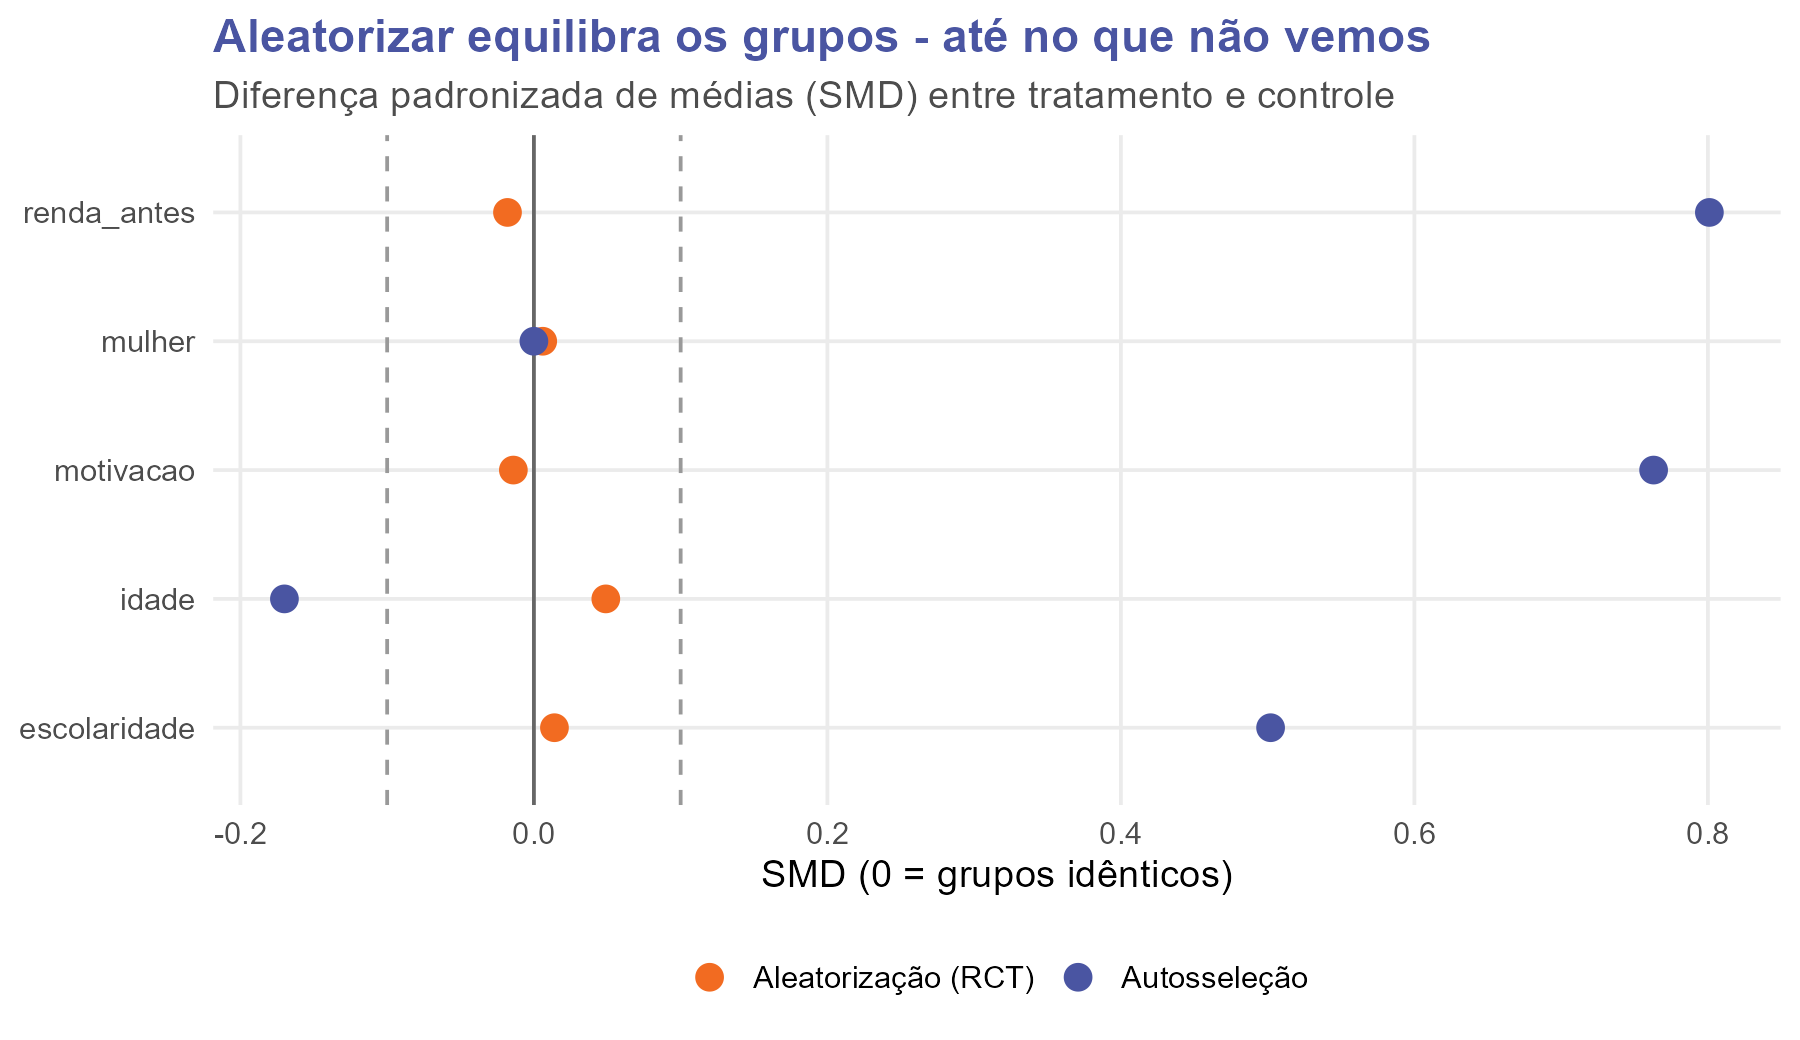
\includegraphics[height=4.4cm]{02_balanco.png}\par
  \footnotesize Com sorteio, até a \ind{motivação} (não observada) fica equilibrada. SMD: diferença padronizada de médias.
\end{frame}

\begin{frame}{Mil avaliações, dois métodos (Monte Carlo)}
  \centering
  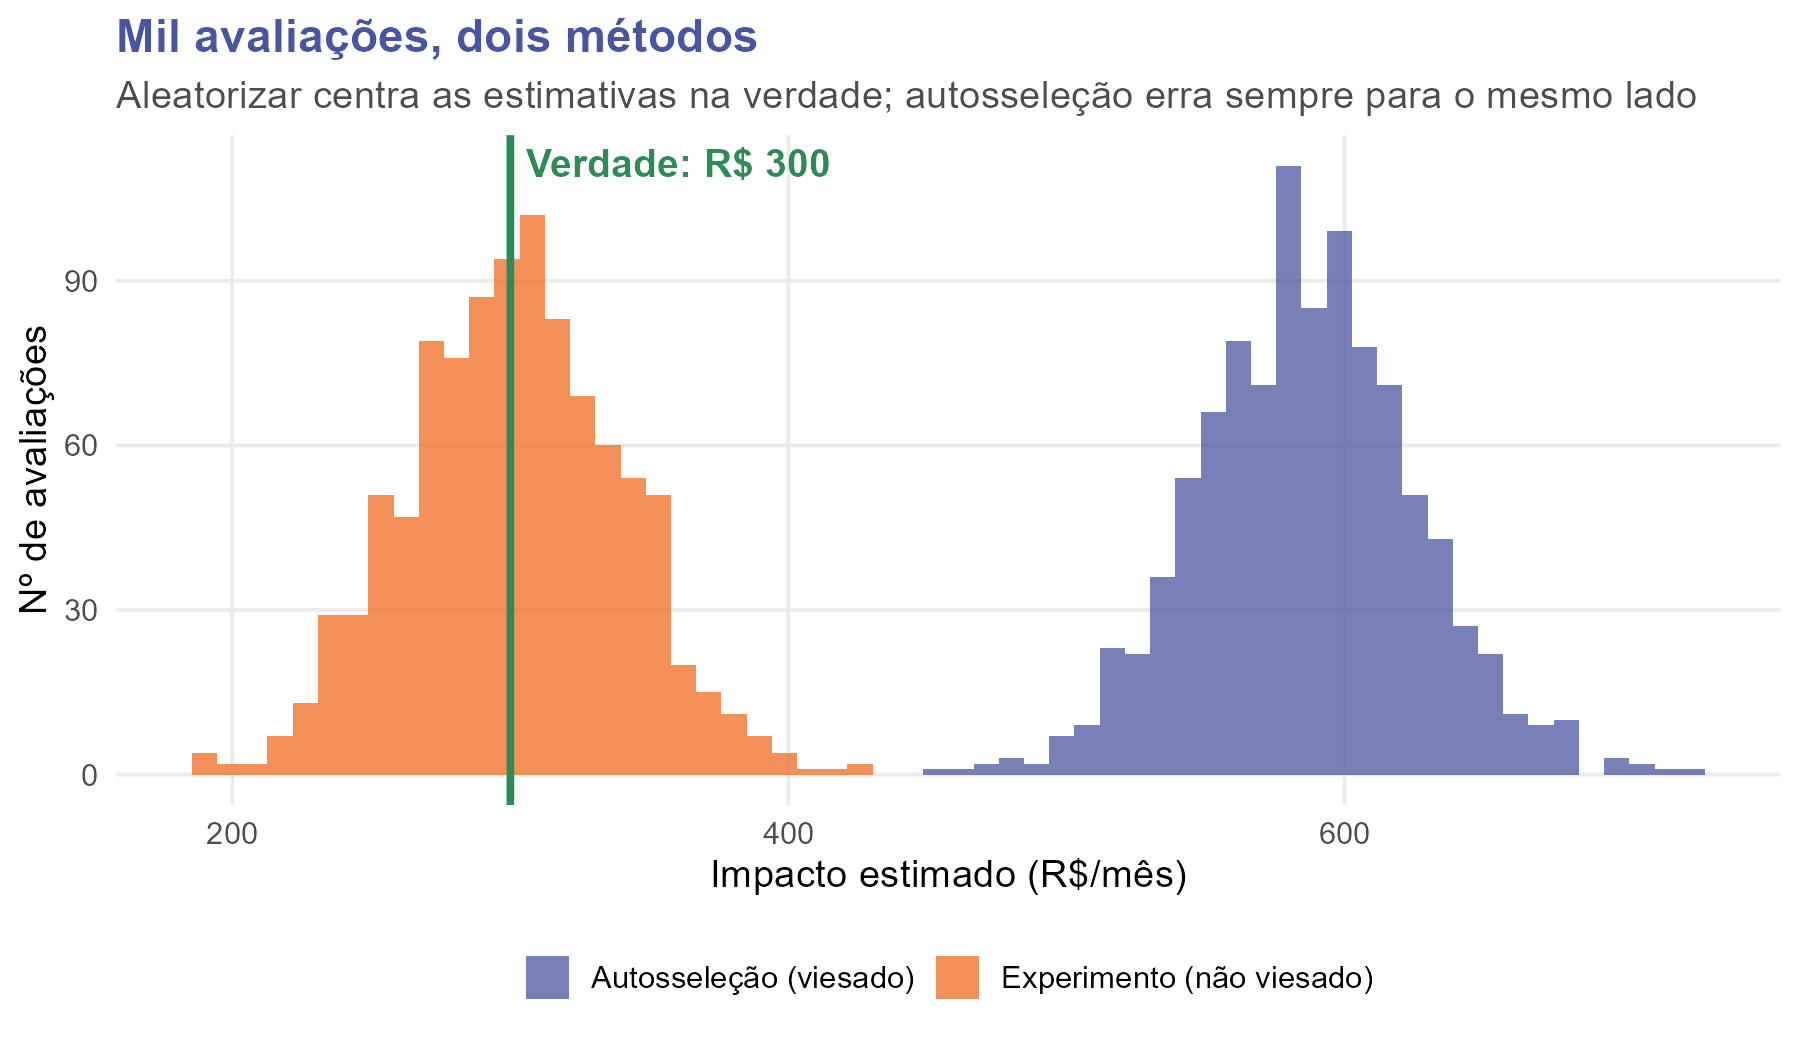
\includegraphics[height=4.3cm]{02_montecarlo.png}\par
  \footnotesize O sorteio acerta \emph{em média} (301); a autosseleção erra \alert{sempre para o mesmo lado} (587). Verdade: 300.
\end{frame}

\begin{frame}{Passo a passo: experimento (1 de 2)}
  \relax{\scriptsize\setlength{\tabcolsep}{2.5pt}\renewcommand{\arraystretch}{1.1}\begin{tabular}{@{}cP{2.55cm}P{2.75cm}P{3.6cm}@{}}
    \toprule
    \cabecalho{Como ler e decidir}
    \linha{1}{Compare tratados e controles \textbf{antes} do programa (SMD)}{idade 0,05\newline mulher 0,01\newline escolaridade 0,01\newline renda antes $-0{,}02$}{Todos $|\text{SMD}|<0{,}10$: o sorteio equilibrou os grupos. \textbf{Siga.} Se não, revise o sorteio.}
    \linha{2}{Estime o efeito: diferença de médias (\cod{t.test}) ou regressão}{efeito = 295,2\newline EP = 11,4\newline IC 95\%: 273 a 318}{Participantes ganham ${\approx}$ R\$ 295 a mais. O IC não inclui zero: efeito \textbf{significativo}.}
    \ultimalinha{3}{Reestime com covariáveis (só para ganhar precisão)}{efeito = 302,1\newline EP = 3,4}{Mesma magnitude, EP três vezes menor. O viés já estava resolvido pelo sorteio.}
  \end{tabular}}
  \caixaconclusao{o Qualifica aumenta a renda em cerca de R\$ 300 (IC 273 a 318). Dados simulados do script 02.}
\end{frame}

\begin{frame}{Passo a passo: experimento (2 de 2)}
  \relax{\scriptsize\setlength{\tabcolsep}{2.5pt}\renewcommand{\arraystretch}{1.1}\begin{tabular}{@{}cP{2.55cm}P{2.75cm}P{3.6cm}@{}}
    \toprule
    \cabecalho{Como ler e decidir}
    \linha{4}{Cheque a \textbf{adesão} (\emph{compliance})}{adesão de 70\%\newline ITT = 193\newline efeito sobre aderentes = 293}{Relate o \textbf{ITT} (efeito da \emph{oferta}) e o efeito sobre quem aderiu.}
    \linha{5}{Cheque o \textbf{atrito}}{3,6\% saíram\newline se saem só os piores: 345}{Compare quem saiu em cada grupo. Atrito seletivo faz o viés voltar.}
    \ultimalinha{6}{Confira o \textbf{poder} (\cod{power.t.test})}{R\$ 300: 34 por grupo\newline R\$ 100: 291 por grupo}{Efeitos pequenos exigem amostras grandes. Calcule \textbf{antes} do experimento.}
  \end{tabular}}
  \caixaconclusao{adesão incompleta e atrito mudam \emph{o que} o número significa.}
\end{frame}

\begin{frame}{Exercício 1: viés de seleção e sorteio (12 min)}
  \begin{exerciciobox}{\texttt{atividades/exercicio\_01\_vies\_e\_experimento.R}}
    \small
    \begin{enumerate}
      \item Varie a força da motivação (0 a 1,5): compare o viés da \textbf{comparação ingênua} com o do \textbf{sorteio};
      \item Quantas pessoas por grupo para detectar R\$ 100 com poder de 90\%?
    \end{enumerate}
  \end{exerciciobox}
  \vspace{0.2cm}
  \textbf{Discutam:} por que o sorteio recupera ${\approx}$ R\$ 300 mesmo quando a motivação pesa muito na inscrição?
\end{frame}

% =============================================================================
% PAREAMENTO / PSM (14:50 a 15:10)   [Script 03]
% =============================================================================
\section[Pareamento]{Pareamento (PSM)}

\begin{frame}{Quando não dá para sortear: pareamento}
  \centering
  \begin{tikzpicture}[scale=0.85,every node/.style={transform shape}]
    \node[font=\footnotesize\bfseries,text=laranja] at (0,2.2) {Participantes};
    \node[font=\footnotesize\bfseries,text=azul] at (6.2,2.2) {Não participantes};
    \node[cxl,minimum width=3cm] (t1) at (0,1.4) {24 anos, 12 de estudo};
    \node[cxl,minimum width=3cm] (t2) at (0,0.2) {41 anos, 9 de estudo};
    \node[cxl,minimum width=3cm] (t3) at (0,-1.0) {35 anos, 14 de estudo};
    \node[cxi,minimum width=3cm] (c1) at (6.2,1.4) {58 anos, 6 de estudo};
    \node[cxi,minimum width=3cm] (c2) at (6.2,0.5) {24 anos, 12 de estudo};
    \node[cxi,minimum width=3cm] (c3) at (6.2,-0.4) {40 anos, 9 de estudo};
    \node[cxi,minimum width=3cm] (c4) at (6.2,-1.3) {35 anos, 14 de estudo};
    \draw[seta] (t1) -- (c2); \draw[seta] (t2) -- (c3); \draw[seta] (t3) -- (c4);
  \end{tikzpicture}
  \vspace{0.2cm}
  \begin{itemize}
    \item Para cada participante, buscar não participantes \ind{parecidos nas características observadas};
    \item Se só o programa os distingue, a diferença \emph{depois} é atribuída à política.
  \end{itemize}
\end{frame}

\begin{frame}{A maldição da dimensionalidade e o escore de propensão}
  \centering
  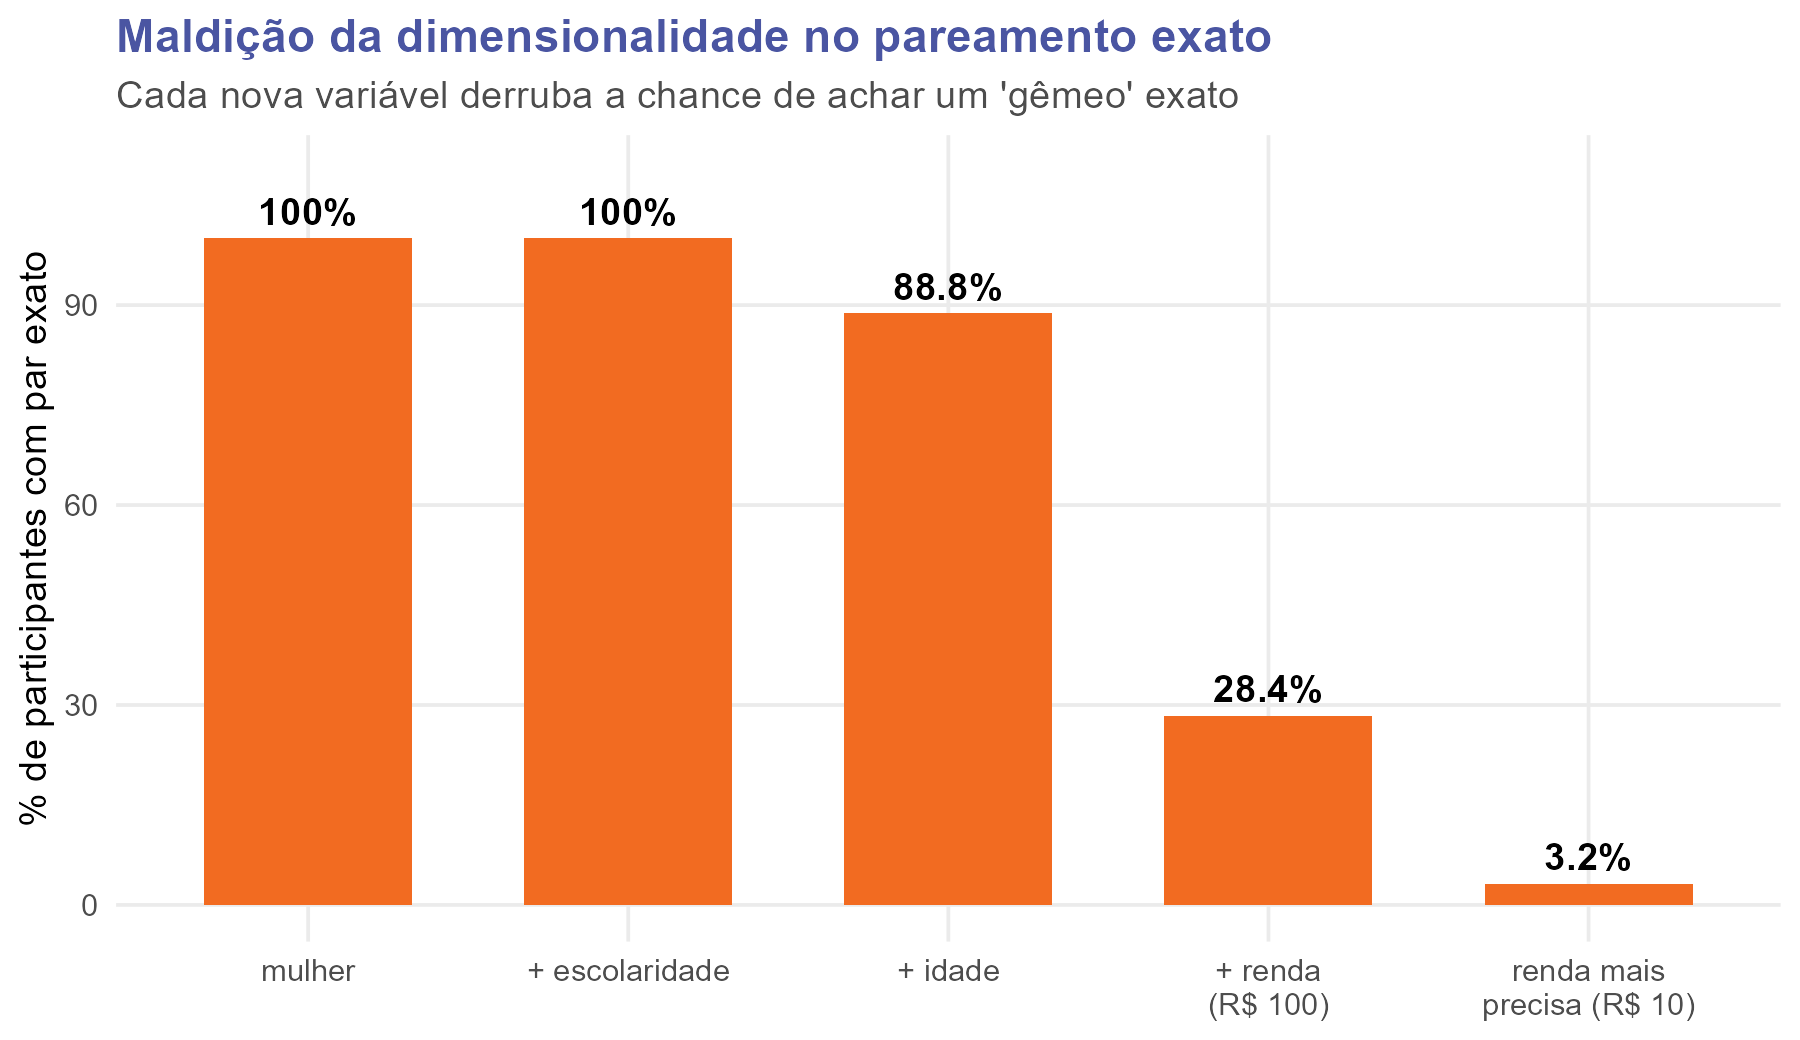
\includegraphics[height=3.9cm]{03_maldicao.png}\par
  \footnotesize Pareamento exato: cada nova variável derruba a chance de achar um ``gêmeo''. \textbf{Solução}: resumir tudo em um número, o \ind{propensity score} (probabilidade de participar), e parear por ele.
\end{frame}

\begin{frame}{Pareamento: características e exemplos}
  \carac{não participantes \textbf{parecidos} (mesmo escore de propensão)}
        {\textbf{sem confundidores não observados}; região comum (há semelhantes nos dois grupos)}
        {efeito sobre os tratados (ATT)}
        {muitas covariáveis \textbf{anteriores} ao programa (idealmente o resultado antes)}
        {política já implementada, sem sorteio, corte ou painel}
  \vspace{0.15cm}
  \textbf{\footnotesize\color{azul}Exemplos em políticas públicas}\par
    \scriptsize
    \begin{itemize}
      \item \textbf{Argentina:} programa de emprego Trabajar durante a crise de 1997 (Jalan e Ravallion, 2003).
      \item \textbf{Brasil:} Bolsa Família, efeitos sobre consumo, educação e saúde (MDS, 2007).
      \item \textbf{EUA:} programa de treinamento profissional reanalisado com PSM (LaLonde, 1986; Dehejia e Wahba, 1999).
      \item \textbf{Hipotético (nosso Qualifica):} programa já implementado, sem sorteio.
    \end{itemize}
  
\end{frame}

\begin{frame}{Passo a passo: pareamento (1 de 2)}
  \relax{\scriptsize\setlength{\tabcolsep}{2.5pt}\renewcommand{\arraystretch}{1.1}\begin{tabular}{@{}cP{2.55cm}P{2.75cm}P{3.6cm}@{}}
    \toprule
    \cabecalho{Como ler e decidir}
    \linha{1}{Compare os grupos \textbf{antes}: diferença simples e balanço (SMD)}{diferença = 587\newline SMD: escolaridade 0,50\newline renda antes 0,80\newline idade $-0{,}17$}{Grupos muito diferentes: a comparação simples \textbf{não vale}. É preciso ajustar.}
    \linha{2}{Estime o escore (logit) e olhe a \textbf{região comum}}{região comum:\newline 0,05 a 0,90}{Ampla sobreposição: há controles para quase todos. Se fosse estreita, o efeito valeria só para poucos.}
    \ultimalinha{3}{Pareie: vizinho mais próximo, \emph{caliper} de 0,2 dp}{1.630 de 1.631 tratados pareados}{Quase todos têm par. Muitos sem par $\Rightarrow$ o efeito vale só para os pareados.}
  \end{tabular}}
\end{frame}

\begin{frame}{Passo a passo: pareamento (2 de 2)}
  \relax{\scriptsize\setlength{\tabcolsep}{2.5pt}\renewcommand{\arraystretch}{1.1}\begin{tabular}{@{}cP{2.55cm}P{2.75cm}P{3.6cm}@{}}
    \toprule
    \cabecalho{Como ler e decidir}
    \linha{4}{\textbf{Balanço depois} do pareamento}{SMD: escolaridade $-0{,}03$\newline idade 0,01; renda antes 0,00\newline motivação 0,30}{Observáveis equilibradas ($<$ 0,10). A \textbf{motivação} (não observada) ainda difere.}
    \linha{5}{Estime o \textbf{ATT} e o intervalo (\emph{bootstrap})}{ATT = 297\newline EP = 8,8\newline IC 95\%: 280 a 315}{Participantes ganham ${\approx}$ R\$ 297 a mais por causa do programa (verdade: 300).}
    \ultimalinha{6}{\textbf{Robustez}: refaça sem a renda antes}{ATT = 476}{Muda muito: depende de uma covariável-chave. Relate e discuta o que pode estar omitido.}
  \end{tabular}}
  \caixaconclusao{o PSM só iguala o que está no modelo.}
\end{frame}

\begin{frame}{Região comum e resultado}
  \begin{columns}[T]
    \begin{column}{0.48\textwidth}
      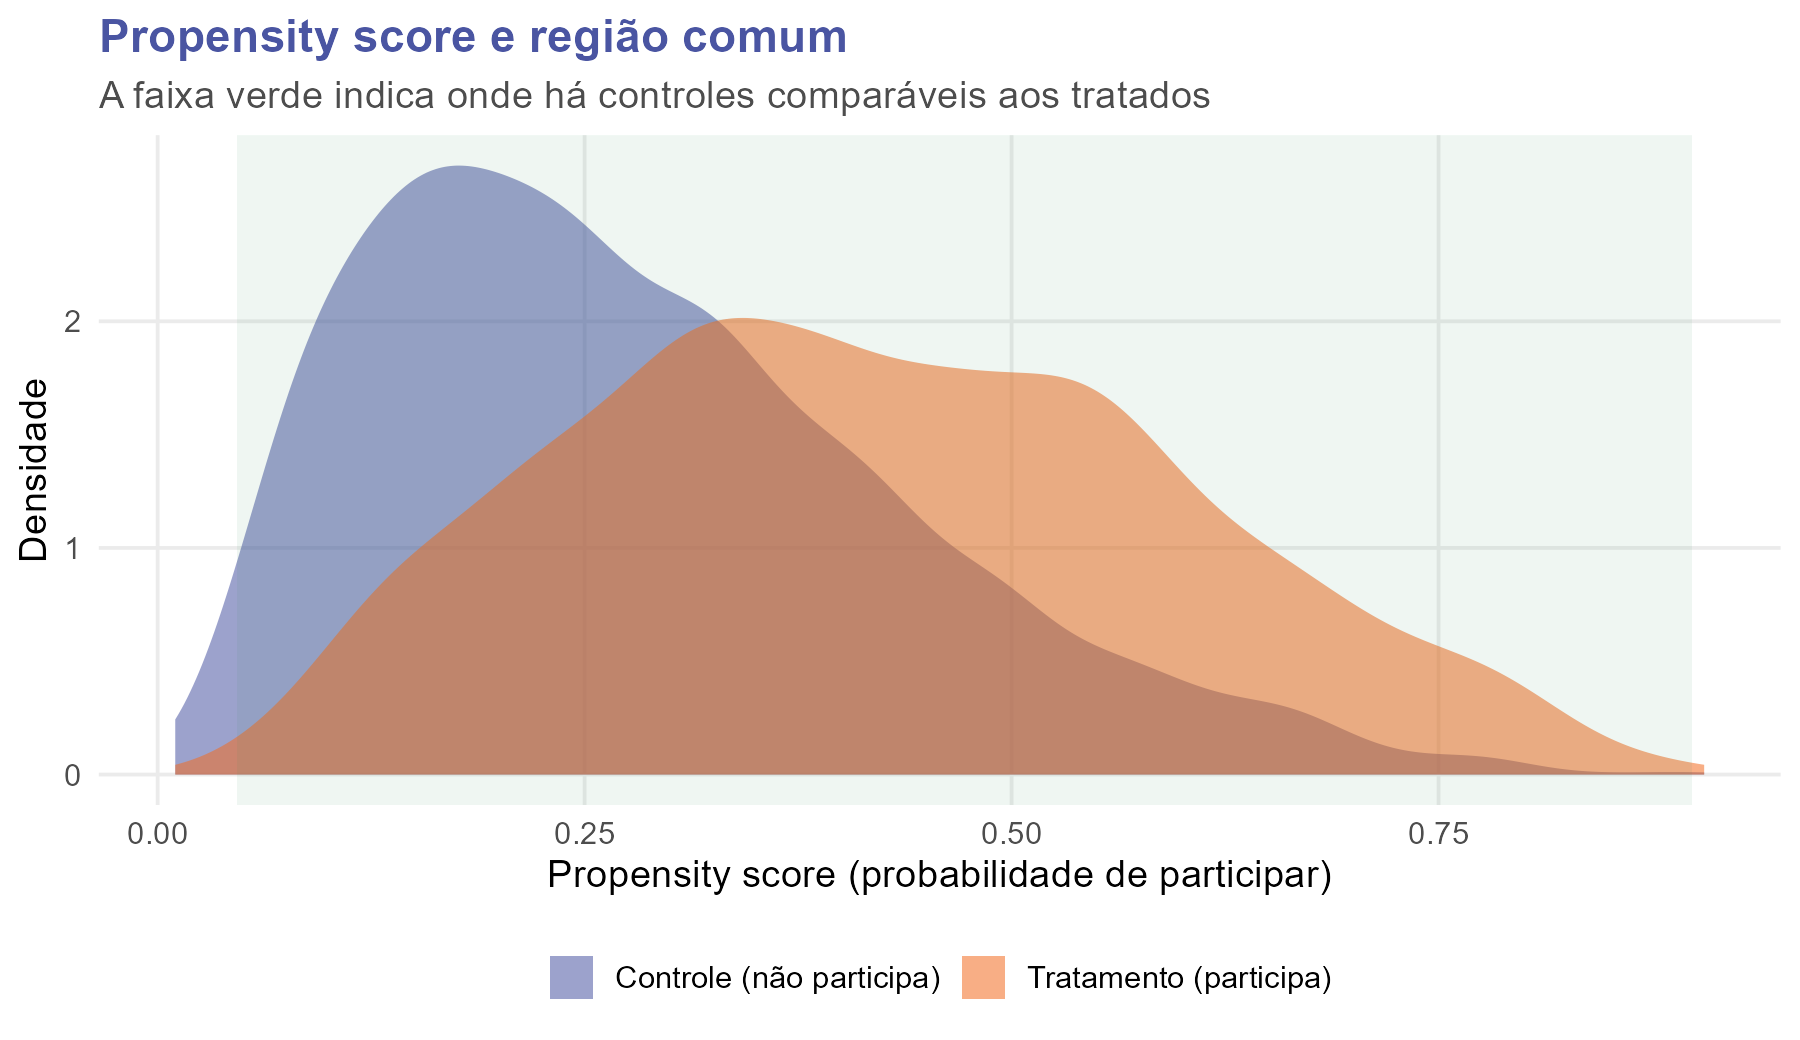
\includegraphics[height=3.2cm]{03_regiao_comum.png}\par
      {\tiny Faixa verde: onde há controles comparáveis.}
    \end{column}
    \begin{column}{0.52\textwidth}
      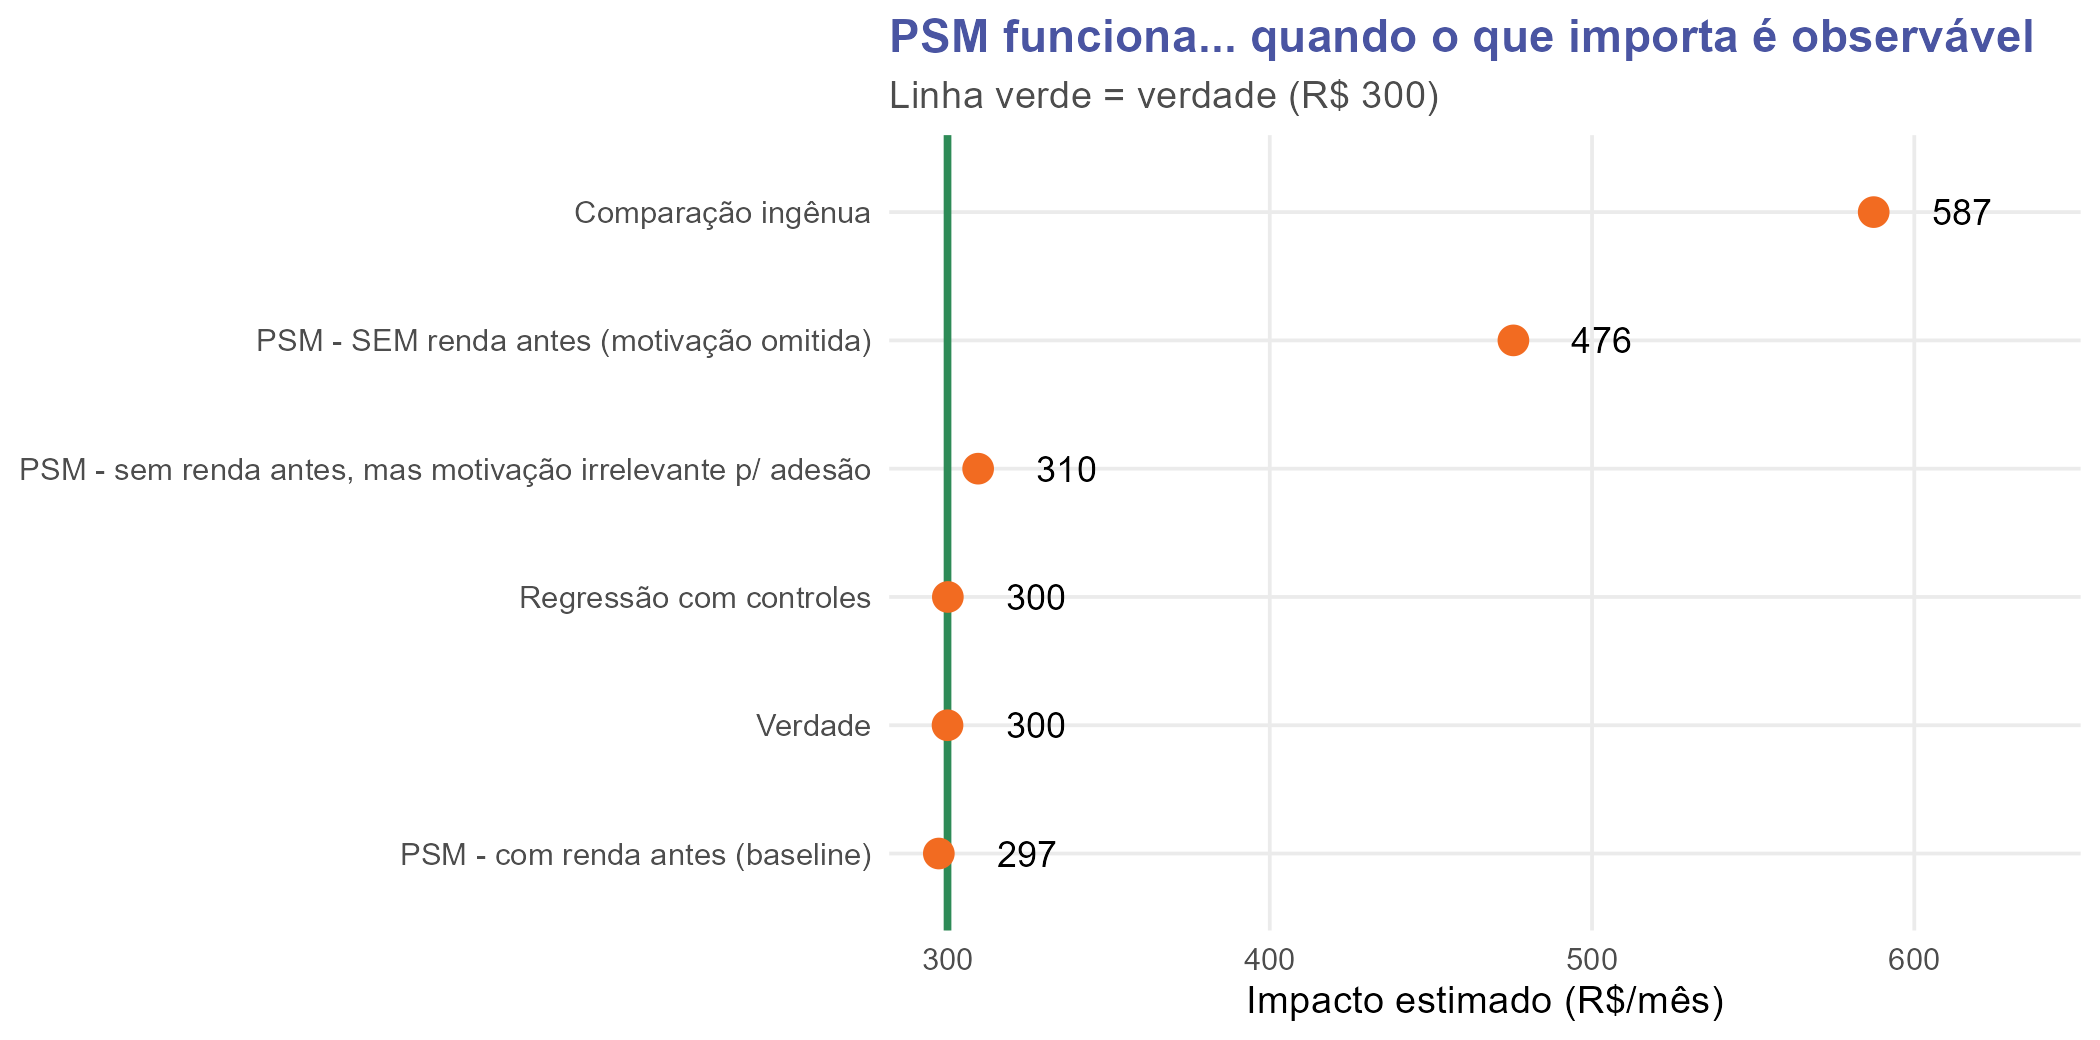
\includegraphics[height=3.2cm]{03_resumo.png}\par
      {\tiny Linha verde: verdade (R\$ 300).}
    \end{column}
  \end{columns}
\end{frame}

% =============================================================================
% DIFERENÇA-EM-DIFERENÇAS (15:10 a 15:35)   [Script 04 | Exercício 2]
% =============================================================================
\section[DiD]{Diferença-em-diferenças}

\begin{frame}{A ideia: comparar variações}
  \begin{block}{Dupla diferença}
    \small
    $$\text{DD}=(\bar Y_{T}^{\,depois}-\bar Y_{T}^{\,antes})-(\bar Y_{C}^{\,depois}-\bar Y_{C}^{\,antes})$$
  \end{block}
  \begin{itemize}
    \item A variação do \textbf{controle} é a tendência que o tratado teria seguido sem a política;
    \item Elimina diferenças \emph{fixas} entre os grupos, mesmo as não observadas;
    \item Pressuposto central: \destaque{tendências paralelas}.
  \end{itemize}
\end{frame}

\begin{frame}{Exemplo numérico}
  \begin{columns}[T]
    \begin{column}{0.4\textwidth}
      \footnotesize
      \renewcommand{\arraystretch}{1.3}
      \begin{tabular}{lrr}
        \toprule
        \textbf{Renda} & \textbf{Part.} & \textbf{Não} \\ \midrule
        Antes & 80 & 90 \\
        Depois & 125 & 120 \\ \midrule
        Variação & +45 & +30 \\ \bottomrule
      \end{tabular}
      \vspace{0.3cm}

      DD $=45-30=$ \destaque{15}\\[4pt]
      {\scriptsize Antes-depois: 45 (superestima). Participantes $\times$ não: 5 (subestima).}
    \end{column}
    \begin{column}{0.6\textwidth}
      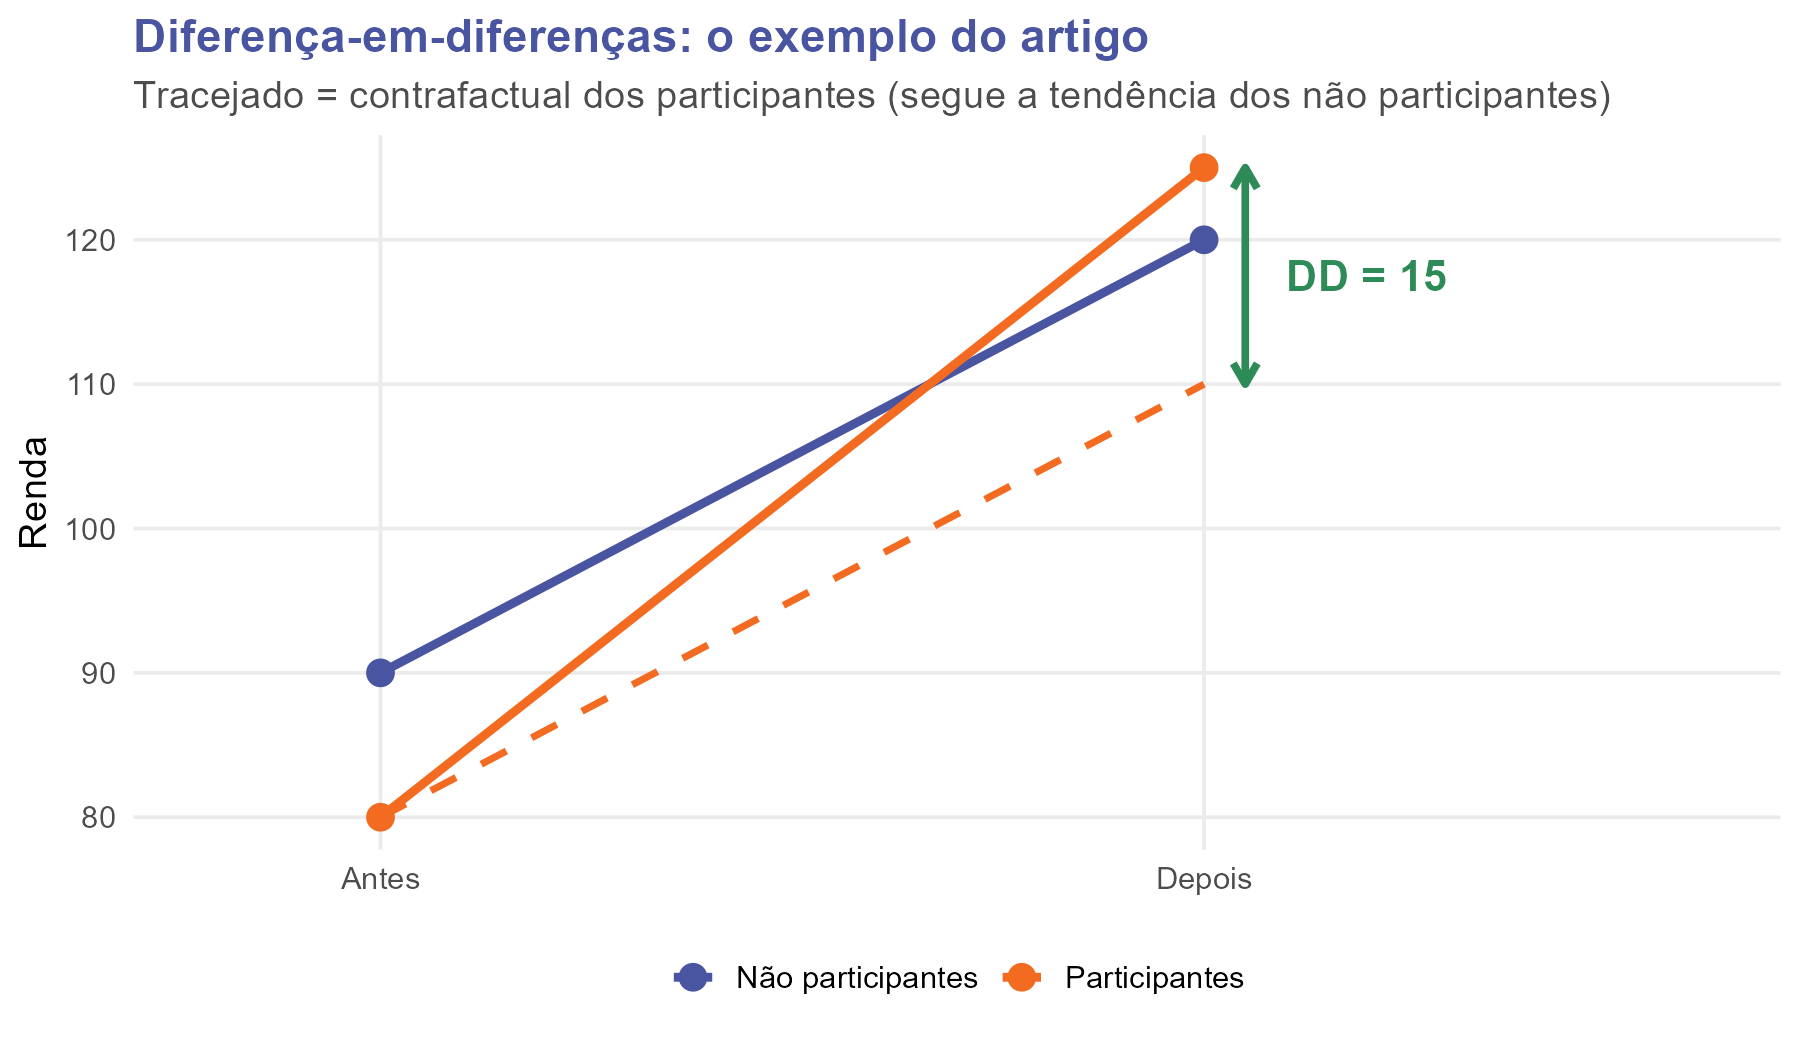
\includegraphics[width=\textwidth]{04_figura6.png}
    \end{column}
  \end{columns}
  \fonte{Exemplo adaptado de Khandker, Koolwal e Samad (2010).}
\end{frame}

\begin{frame}{Diferença-em-diferenças: características e exemplos}
  \carac{a \textbf{tendência do grupo de controle} aplicada ao tratado}
        {\textbf{tendências paralelas} na ausência da política; sem antecipação; sem contaminação}
        {efeito sobre os tratados (ATT)}
        {dados \textbf{antes e depois} de tratados e controles (painel ou cortes repetidos)}
        {política implantada só em parte do território ou da população; leis}
  \vspace{0.15cm}
  \textbf{\footnotesize\color{azul}Exemplos em políticas públicas}\par
    \scriptsize
    \begin{itemize}
      \item \textbf{Brasil:} Lei Maria da Penha. Mulheres (tratamento) $\times$ homens (controle), taxa de homicídios (Cerqueira et al., 2015).
      \item \textbf{EUA:} aumento do salário mínimo em Nova Jersey, com lanchonetes da Pensilvânia como controle (Card e Krueger, 1994).
      \item \textbf{Hipotético:} bolsa-permanência em algumas escolas (Exercício 2); Qualifica numa região (script 04).
    \end{itemize}
  
\end{frame}

\begin{frame}{Simulação: tendências paralelas antes do programa}
  \centering
  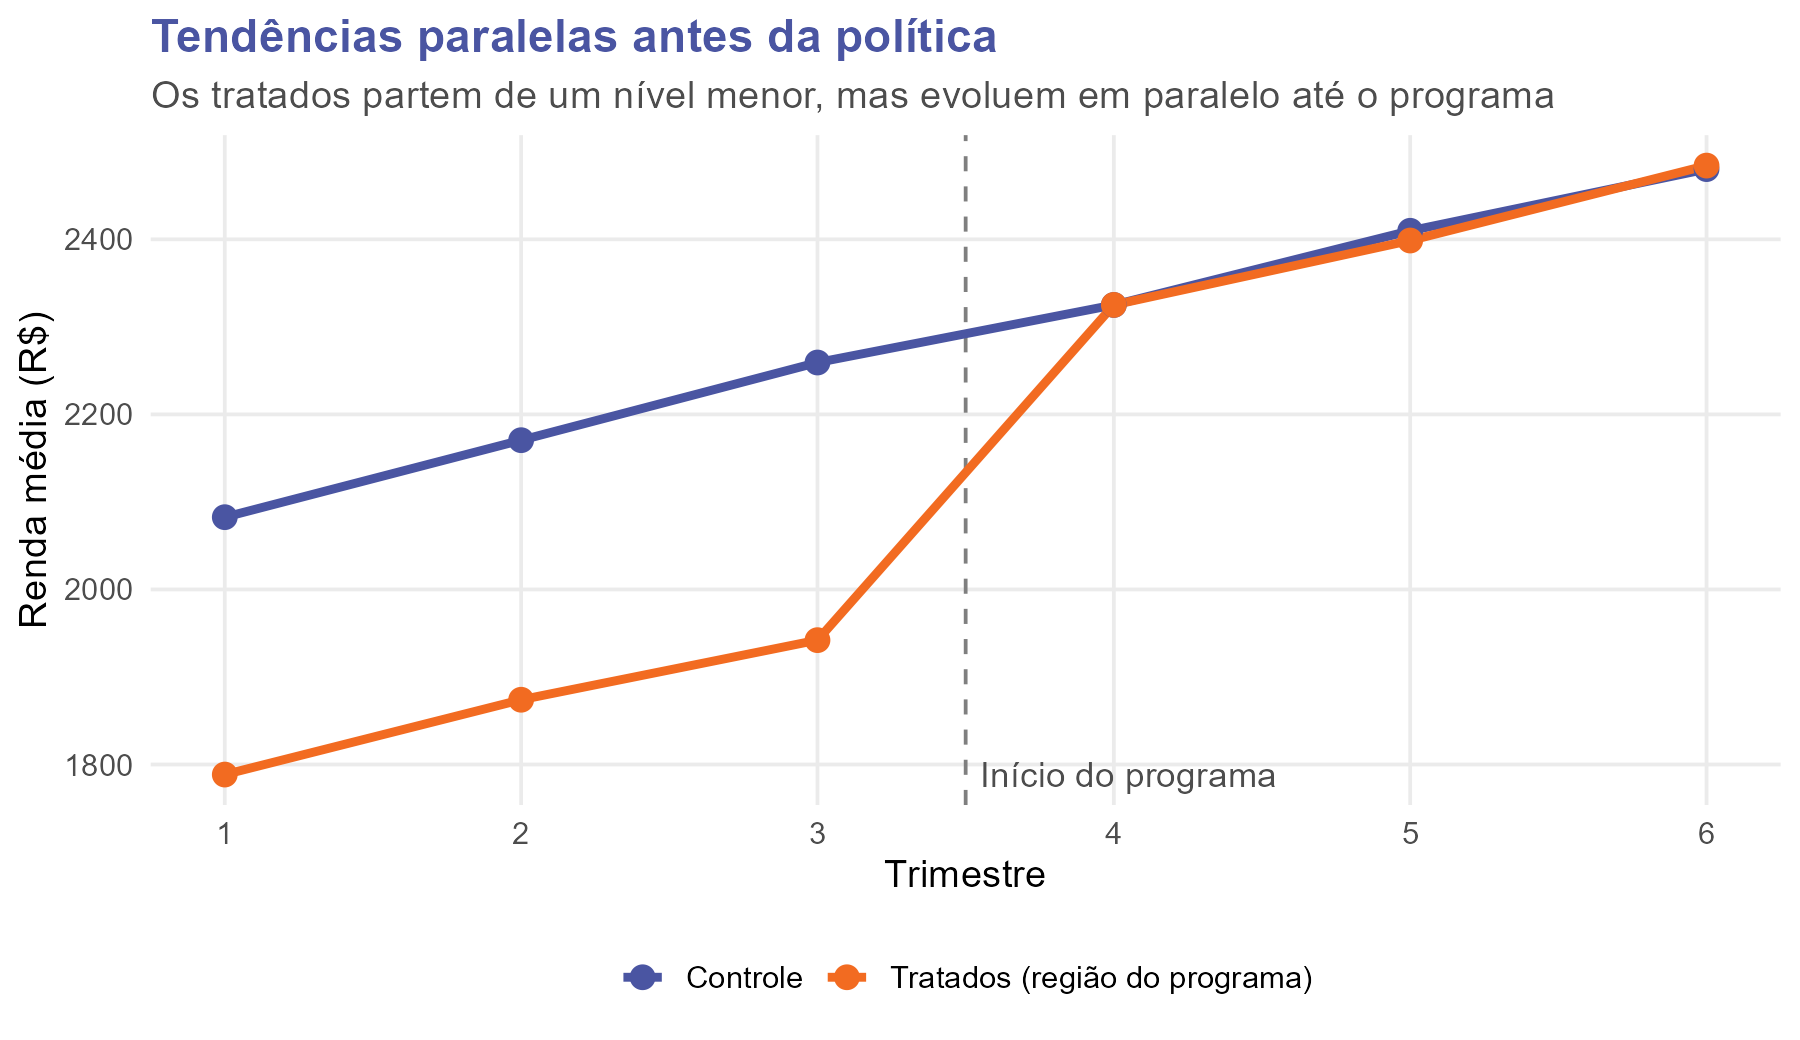
\includegraphics[height=3.9cm]{04_tendencias.png}\par
  \footnotesize Os tratados partem de um nível menor (mais pobres), mas \textbf{evoluem em paralelo} até o 4.º trimestre, quando começa o programa.
\end{frame}

\begin{frame}{Passo a passo: diferença-em-diferenças (1 de 2)}
  \relax{\scriptsize\setlength{\tabcolsep}{2.5pt}\renewcommand{\arraystretch}{1.1}\begin{tabular}{@{}cP{2.55cm}P{2.75cm}P{3.6cm}@{}}
    \toprule
    \cabecalho{Como ler e decidir}
    \linha{1}{Olhe as tendências \textbf{antes} da política}{tratados: 1.789; 1.874; 1.942\newline controle: 2.083; 2.171; 2.259}{Sobem ${\approx}$ +80 por trimestre nos dois: \textbf{paralelas}.}
    \linha{2}{Calcule as \textbf{4 médias} (antes/depois, tratado/controle)}{tratados: 1.868 $\to$ 2.403 (+534)\newline controle: 2.171 $\to$ 2.405 (+234)}{Os dois sobem. A variação do controle (+234) é a tendência.}
    \ultimalinha{3}{\textbf{Dupla diferença}}{DD = 534 $-$ 234 = 300}{O programa elevou a renda em R\$ 300 \textbf{além da tendência}. (Antes-depois: 534.)}
  \end{tabular}}
\end{frame}

\begin{frame}{Passo a passo: diferença-em-diferenças (2 de 2)}
  \relax{\scriptsize\setlength{\tabcolsep}{2.5pt}\renewcommand{\arraystretch}{1.1}\begin{tabular}{@{}cP{2.55cm}P{2.75cm}P{3.6cm}@{}}
    \toprule
    \cabecalho{Como ler e decidir}
    \linha{4}{Regressão com \textbf{interação} e erro-padrão por \emph{cluster}}{tratado:pos = 300,2\newline EP = 7,8\newline IC 95\%: 285 a 315}{Mesmo número do passo 3, agora com incerteza.}
    \linha{5}{\textbf{Estudo de eventos}: efeito por trimestre (ref.: 3.º)}{antes: +23 e +21 (EP 34)\newline depois: 317, 306, 321}{Antes ${\approx}$ 0 (sem pré-tendência). Depois ${\approx}$ 300, estável.}
    \ultimalinha{6}{\textbf{Placebo}: finja o programa mais cedo}{DD placebo = $-13$}{Perto de zero: ok. Se fosse grande (no cenário ruim: +47), \textbf{desconfie}.}
  \end{tabular}}
  \caixaconclusao{DD = R\$ 300 (verdade: 300), com tendências paralelas confirmadas por dois testes.}
\end{frame}

\begin{frame}{Quando as tendências \textit{não} são paralelas}
  \centering
  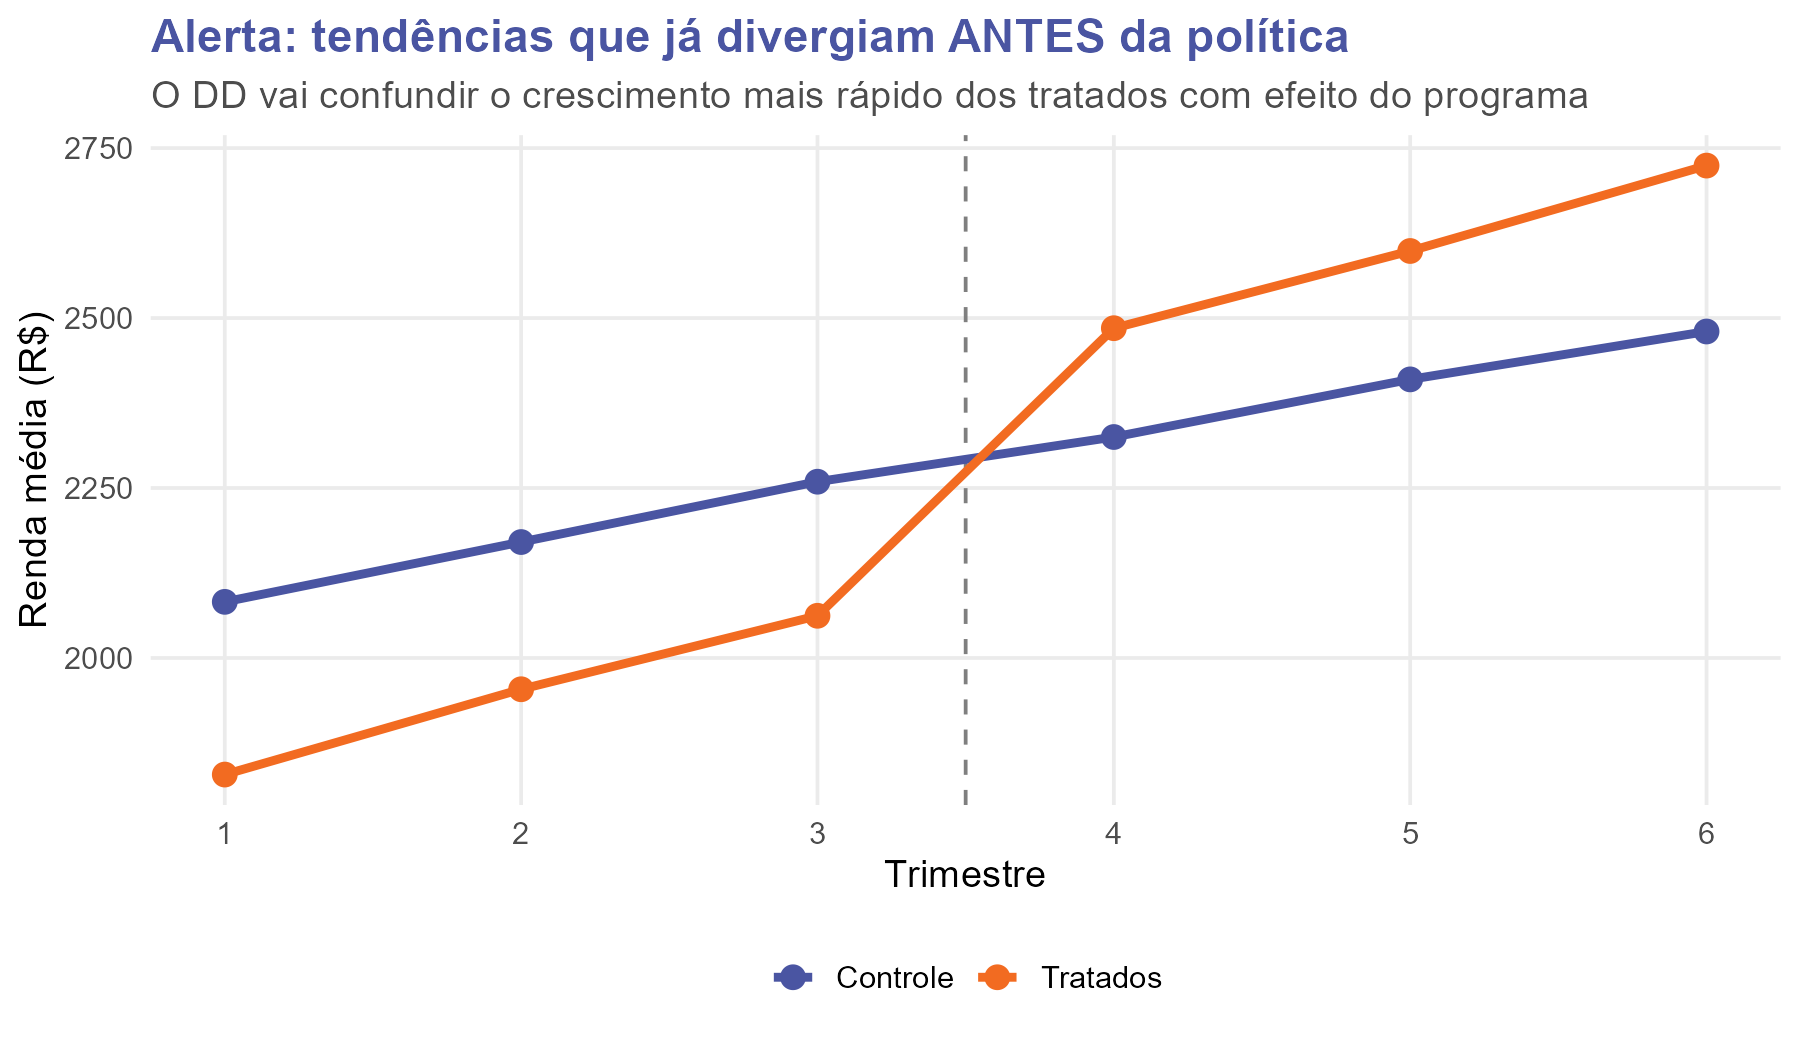
\includegraphics[height=4.0cm]{04_nao_paralelas.png}\par
  \footnotesize Os tratados já cresciam mais rápido: o DD estima \alert{R\$ 420} (verdade: 300). O \textbf{placebo} denuncia o problema: +47.
\end{frame}

\begin{frame}{Exercício 2: diferença-em-diferenças (10 min)}
  \begin{exerciciobox}{\texttt{atividades/exercicio\_02\_diferenca\_em\_diferenca.R}}
    \small
    \begin{enumerate}
      \item Calcule o DD de uma bolsa-permanência (evasão de 12\% para 8\% nas escolas com programa; de 10\% para 9\% nas demais);
      \item Gere um painel com tendência extra de R\$ 20/trimestre para os tratados: o DD acerta? O placebo avisa?
    \end{enumerate}
  \end{exerciciobox}
  \vspace{0.2cm}
  \textbf{Para pensar (Lei Maria da Penha):} que evento poderia afetar mulheres e homens de forma diferente e violar as tendências paralelas?
\end{frame}

% =============================================================================
% REGRESSÃO DESCONTÍNUA (15:15 a 15:30)   [Script 05]
% =============================================================================
\section[RDD]{Regressão descontínua}
\subsection{Ideia e exemplos}

\begin{frame}{A ideia: um ``experimento natural'' no corte}
  \begin{itemize}
    \item Muitos programas têm uma \ind{regra de elegibilidade}: um índice contínuo e um \textbf{ponto de corte};
    \item Ex.: transferência de renda para quem tem renda per capita \textbf{até R\$ 77}. Uma família com R\$ 77 recebe; outra com R\$ 78, não;
    \item Perto do corte, as famílias são muito parecidas: é \destaque{como se houvesse um sorteio};
    \item O impacto é o tamanho do \ind{salto} no corte.
  \end{itemize}
\end{frame}

\begin{frame}{Regressão descontínua: características e exemplos}
  \carac{famílias \textbf{logo do outro lado do corte}}
        {\textbf{continuidade}: sem manipulação do corte e sem outros saltos no mesmo ponto}
        {efeito \textbf{local}, para quem está no corte}
        {índice contínuo, corte claro e \textbf{muitas observações} perto dele}
        {programas com elegibilidade por escore (renda, nota, idade, população)}
  \vspace{0.05cm}
  \textbf{\footnotesize\color{azul}Exemplos em políticas públicas}\par
    \scriptsize
    \begin{itemize}
      \item \textbf{México:} elegibilidade do Progresa e frequência escolar (Buddelmeyer e Skoufias, 2004).
      \item \textbf{Israel:} turmas divididas quando passam de 40 alunos (regra de Maimônides) e desempenho (Angrist e Lavy, 1999).
      \item \textbf{Eleições:} candidatos eleitos por margem mínima (Lee, 2008).
    \end{itemize}
\end{frame}

\begin{frame}{A descontinuidade no corte}
  \centering
  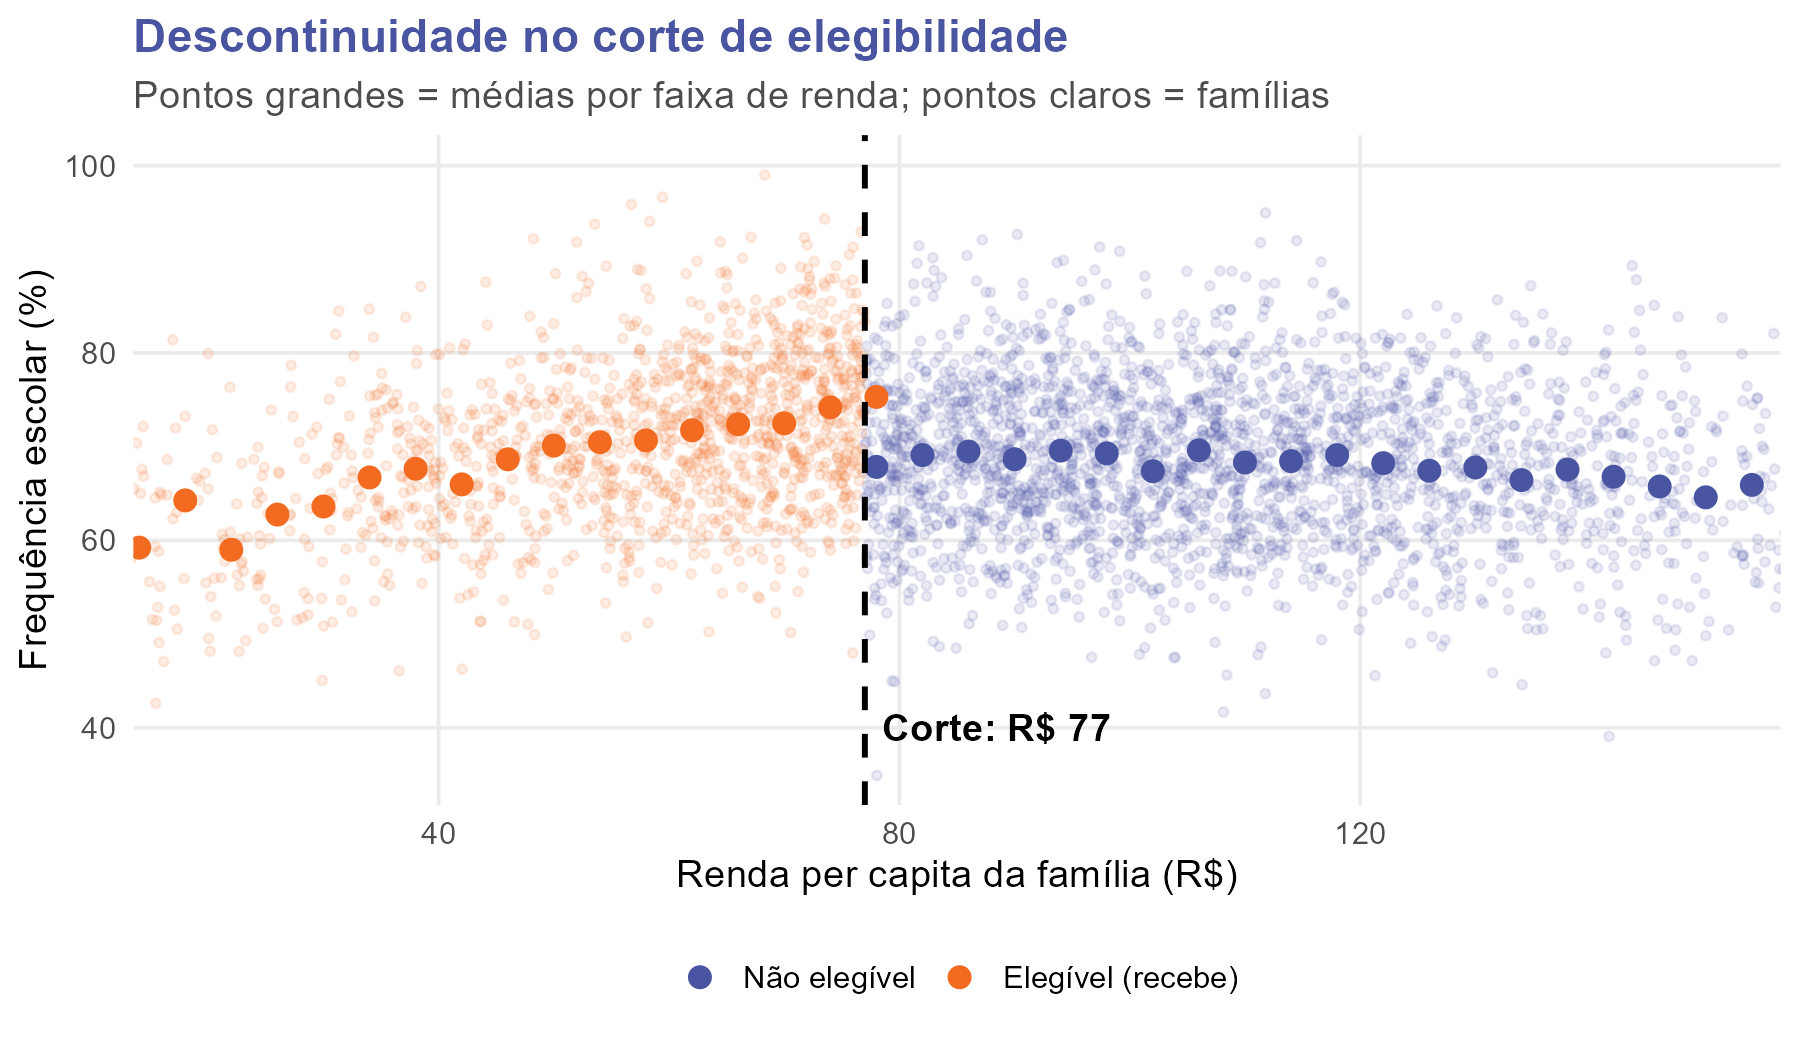
\includegraphics[height=4.2cm]{05_rdd_dispersao.png}\par
  \footnotesize Pontos grandes: médias por faixa de R\$ 4. Elegíveis (laranja) têm frequência escolar maior logo abaixo do corte.
\end{frame}

\subsection{Passo a passo}

\begin{frame}[fragile]{RDD, passo 1: de quanto é o salto no corte?}
\begin{consoleR}
@@> rd <- rdrobust(y = d$freq, x = -d$x)
@@> with(rd, round(data.frame(efeito = coef[1], ep = se[1],
@@+       ic_inf = ci[3, 1], ic_sup = ci[3, 2],
@@+       h = bws[1, 1]), 2))
  efeito   ep ic_inf ic_sup     h
1   6.75 0.93   5.03   9.19 16.78
\end{consoleR}
\begin{leitura}
  \begin{itemize}\setlength{\itemsep}{1pt}
    \item \rot{Onde olhar:} o \texttt{rdrobust} escolhe a janela sozinho (\texttt{h} $=16{,}8$) e estima o salto: \destaque{6,75 pontos} de frequência escolar (verdade: 6), EP 0,93. Usamos \texttt{x = -d\$x} porque os elegíveis estão \emph{abaixo} do corte.
    \item \rot{Corte:} IC robusto de 5,0 a 9,2, sem zero (Calonico, Cattaneo e Titiunik, 2014).
  \end{itemize}
\end{leitura}
\end{frame}

\begin{frame}[fragile]{RDD, passo 2: o resultado depende da janela?}
\begin{consoleRpeq}
@@> t(sapply(c(5, 15, 40), function(h) {
@@+   r <- rdrobust(d$freq, -d$x, h = h)
@@+   round(c(h = h, efeito = r$coef[1], ep = r$se[1],
@@+           controle = r$N_h[1], tratamento = r$N_h[2]), 2)
@@+ }))
      h efeito   ep controle tratamento
[1,]  5   7.21 1.59      227        213
[2,] 15   6.95 0.98      655        616
[3,] 40   5.79 0.64     1684       1149
\end{consoleRpeq}
\begin{leitura}
  \begin{itemize}\setlength{\itemsep}{1pt}
    \item \rot{Onde olhar:} \texttt{h} é a janela em R\$; \texttt{controle} e \texttt{tratamento} são as famílias de cada lado dentro dela. O efeito fica entre 5,8 e 7,2: não depende da janela.
    \item \rot{Corte:} mostrar várias janelas (Lee e Lemieux, 2010).
  \end{itemize}
\end{leitura}
\end{frame}

\begin{frame}[fragile]{RDD, passo 3: os dois lados do corte são comparáveis?}
\begin{consoleR}
@@> rc <- rdrobust(d$idade_mae, -d$x)
@@> round(c(salto = rc$coef[1], ep = rc$se[1],
@@+         p = rc$pv[3]), 2)
salto    ep     p
-0.13  0.76  0.85
@@> rd_dens <- rddensity(-d$x)
@@> round(rd_dens$test$p_jk, 3)
[1] 0.967
\end{consoleR}
\begin{leitura}
  \begin{itemize}\setlength{\itemsep}{1pt}
    \item \rot{Onde olhar:} (1) a idade da mãe não deve ``saltar'': salto $-0{,}13$, $p=0{,}85$. (2) a densidade da renda não deve ter salto: $p=0{,}97$, sem acúmulo logo abaixo do corte.
    \item \rot{Corte:} aqui queremos $p$ \emph{alto} (Cattaneo, Jansson e Ma, 2020).
  \end{itemize}
\end{leitura}
\end{frame}

\begin{frame}{Teste de manipulação}
  \centering
  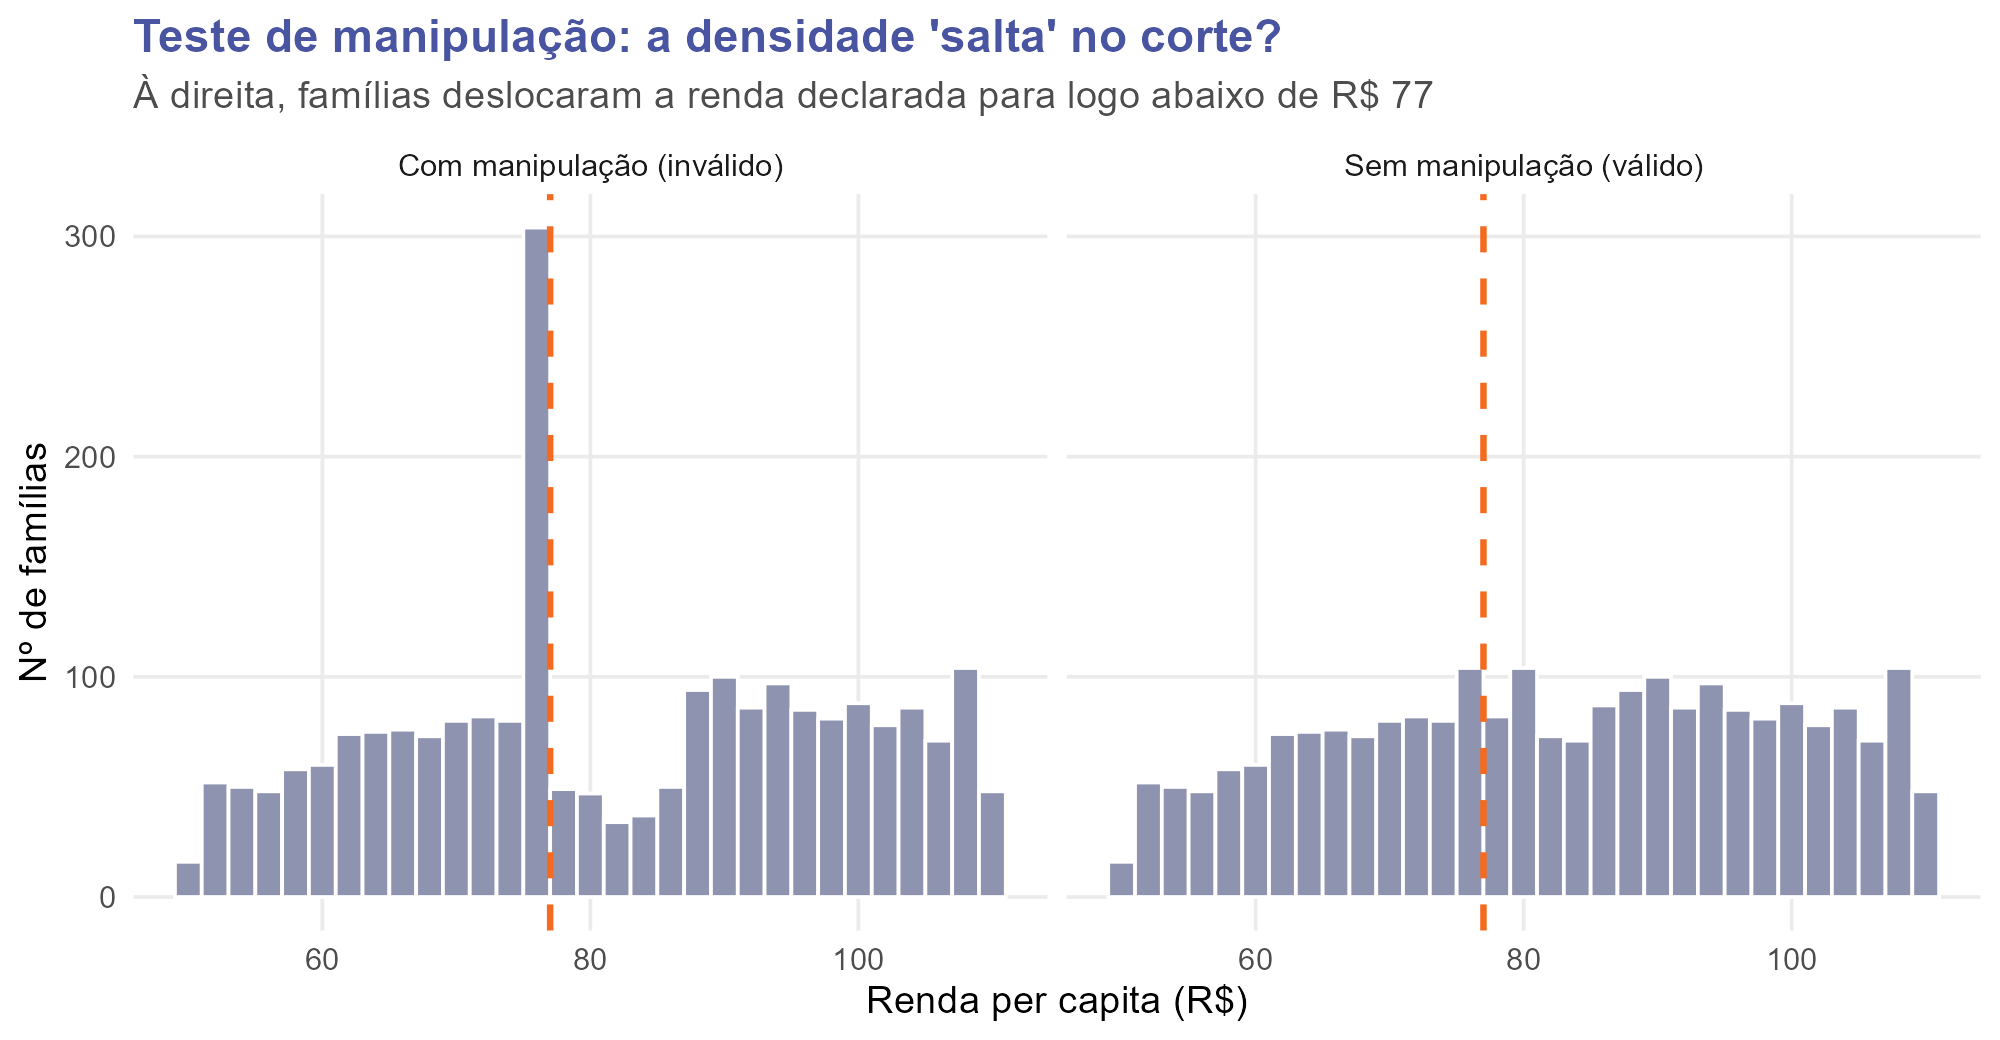
\includegraphics[height=3.7cm]{05_rdd_manipulacao.png}\par
  \footnotesize À esquerda, famílias deslocaram a renda declarada para logo abaixo de R\$ 77: o RDD perde a validade.
\end{frame}

% =============================================================================
% BLOCO 6 — TÉCNICAS QUALITATIVAS E MÉTODOS MISTOS  (17:05–17:50)   [Atividade 6]
% =============================================================================
\secao{Bloco 6}{Técnicas qualitativas e métodos mistos}{17:05 -- 17:50 \,$\cdot$\, Atividade 6}

\begin{frame}{Quantificar o impacto $\times$ compreender o impacto}
  \begin{columns}[T]
    \begin{column}{0.5\textwidth}
      \begin{block}{Abordagem quantitativa}
        \small
        \begin{itemize}
          \item \textbf{Quanto?} Magnitude do \emph{efeito médio};
          \item Foco no que é \emph{geral}, comum;
          \item Lida com viés de seleção; busca o contrafactual;
          \item Generalização, replicação, transparência dos métodos.
        \end{itemize}
      \end{block}
    \end{column}
    \begin{column}{0.5\textwidth}
      \begin{atividadebox}{Abordagem qualitativa}
        \small
        \begin{itemize}
          \item \textbf{Como e por quê?} Qualidade da mudança;
          \item Foco no que é \emph{específico}, no contexto e nos \textbf{significados} que os atores atribuem;
          \item Poucos casos, em profundidade;
          \item Valores, símbolos, percepções.
        \end{itemize}
      \end{atividadebox}
    \end{column}
  \end{columns}
  \vspace{0.2cm}
  \begin{center}\small ``Respondem a diferentes questões'': o quantitativo \emph{identifica}, o qualitativo \emph{explica}.\end{center}
  \fonte{Batista e Domingos (2017), pp.~13--14, a partir de Patton (2002).}
\end{frame}

\begin{frame}{Por que incluir a perspectiva dos atores?}
  \begin{enumerate}
    \item Parte da \ind{perspectiva dos atores} para \textbf{reconstruir a política} (como foi implementada e percebida);
    \item Identifica \ind{impactos diferenciados} sobre diferentes grupos e indivíduos;
    \item Analisa \ind{dimensões não diretamente quantificáveis} (ex.: empoderamento, capital social);
    \item Explica \ind{por que} em algumas situações as políticas atingem os objetivos e em outras não: ajuda a ``abrir a caixa-preta''.
  \end{enumerate}
  \vspace{0.3cm}
  \begin{block}{Uma metáfora do artigo (Patton, 2002)}
    \small Se você quer saber \emph{quanto} pesam as pessoas, use uma balança. Se quer saber \emph{o que o peso significa} para elas, é preciso ouvir suas histórias.
  \end{block}
  \fonte{Batista e Domingos (2017), pp.~14--15.}
\end{frame}

\begin{frame}{Observação e etnografia}
  \begin{columns}[T]
    \begin{column}{0.55\textwidth}
      \small
      \begin{itemize}
        \item \textbf{Imersão} do pesquisador na cultura/grupo; notas de campo, descrições densas, contexto;
        \item \textbf{Participante} (torna-se membro funcional) ou \textbf{não participante} (apenas observa);
        \item O \ind{tempo} é fator central: observações curtas geram interpretações parciais; longos períodos reduzem a \emph{reflexividade} (o observado se comporta ``diferente'' na presença do pesquisador);
        \item Na avaliação: como a política é percebida no cotidiano e \emph{como as pessoas reagem aos seus instrumentos}.
      \end{itemize}
    \end{column}
    \begin{column}{0.45\textwidth}
      \begin{block}{Adato (2008): PTCRs na Nicarágua e na Turquia}
        \footnotesize
        Surveys + etnografia + entrevistas. O survey dizia que o programa era bem \emph{focalizado}, mas a \textbf{comunidade percebia o critério como arbitrário}; mães não davam o suplemento de ferro às crianças por julgarem que \emph{fazia mal}; crianças eram superalimentadas antes da pesagem obrigatória para ``passar no teste''.
      \end{block}
    \end{column}
  \end{columns}
  \fonte{Batista e Domingos (2017), pp.~15--16.}
\end{frame}

\begin{frame}{Entrevistas em profundidade}
  \begin{columns}[T]
    \begin{column}{0.55\textwidth}
      \begin{itemize}
        \item A \emph{palavra} do participante é o foco; perguntas \textbf{abertas e flexíveis}, em oposição aos questionários fechados;
        \item Tipos: \textbf{estruturada}, \textbf{semiestruturada} (tópicos-guia), \textbf{não estruturada} e \textbf{narrativa};
        \item O entrevistador precisa construir \ind{confiança} e preparar um tópico-guia com progressão lógica;
        \item Útil para aprofundar um tema, mapear percepções individuais ou temas \emph{sensíveis}.
      \end{itemize}
    \end{column}
    \begin{column}{0.45\textwidth}
      \begin{block}{Patton (2002): programa de alfabetização de adultos}
        \footnotesize
        O survey registrou que \textbf{77\% estavam ``muito satisfeitos''}. As entrevistas mostraram \emph{por quê}: ler os frascos de remédio das crianças, ler a Bíblia, fazer compras --- ênfase no \textbf{empoderamento} cotidiano, não na colocação no mercado de trabalho (objetivo principal do programa).
      \end{block}
    \end{column}
  \end{columns}
  \fonte{Batista e Domingos (2017), pp.~16--17.}
\end{frame}

\begin{frame}{Grupos focais}
  \begin{columns}[T]
    \begin{column}{0.55\textwidth}
      \begin{itemize}
        \item \textbf{Não} é a soma de entrevistas individuais: o foco está na \ind{discussão e deliberação} entre os participantes;
        \item O moderador \emph{fomenta} a discussão, limita dominantes, incentiva quem fala pouco e mantém o tema;
        \item Bom para explorar o \emph{espectro} de atitudes e opiniões e observar \textbf{consenso e divergência}.
      \end{itemize}
    \end{column}
    \begin{column}{0.45\textwidth}
      \begin{block}{Hunter e Sugiyama (2014): Bolsa Família}
        \footnotesize
        11 grupos focais em 3 municípios do Nordeste (Camaragibe, Jaboatão dos Guararapes e Pau-Brasil) + entrevistas com gestores. Sugerem que o programa deu \textbf{dignidade} às famílias (compra de comida, roupas e material escolar), autonomia frente ao clientelismo e senso de \textbf{empoderamento}.
      \end{block}
    \end{column}
  \end{columns}
  \fonte{Batista e Domingos (2017), pp.~17--18.}
\end{frame}

\begin{frame}{Críticas comuns --- e cuidados}
  \begin{columns}[T]
    \begin{column}{0.5\textwidth}
      \begin{block}{Críticas}
        \small
        \begin{itemize}
          \item \alert{Subjetividade} e especificidade dos resultados;
          \item Ausência de \emph{regularidades} ou generalização;
          \item Menor precisão;
          \item Dificuldade de \emph{replicação}.
        \end{itemize}
      \end{block}
    \end{column}
    \begin{column}{0.5\textwidth}
      \begin{block}{Cuidados e respostas}
        \small
        \begin{itemize}
          \item \textbf{Representatividade} como \ind{variabilidade} (incluir posições diferentes), não como probabilidade estatística;
          \item Selecionar casos usando evidência \emph{quantitativa} (evita viés);
          \item Tempo de campo, treinamento do entrevistador, tópico-guia;
          \item Menos intrusiva: considera a percepção dos próprios atores.
        \end{itemize}
      \end{block}
    \end{column}
  \end{columns}
  \fonte{Batista e Domingos (2017), pp.~14, 18--19.}
\end{frame}

\begin{frame}{Combinando métodos: o que se ganha}
  \begin{columns}[T]
    \begin{column}{0.5\textwidth}
      \begin{enumerate}
        \item \textbf{Validade e credibilidade}: convergência ao medir o mesmo fenômeno (\emph{triangulação});
        \item \textbf{Compreensividade}: capta diferentes dimensões sob perspectivas distintas;
        \item \textbf{Descoberta} de fatores inesperados;
        \item \textbf{Diversidade} de olhares.
      \end{enumerate}
    \end{column}
    \begin{column}{0.5\textwidth}
      \begin{beamercolorbox}[wd=\textwidth,rounded=true,sep=0.3cm]{laranjabox}
        \small
        \textbf{Regra de ouro:} nenhum método é sempre o mais apropriado. O método deve ser escolhido pela \textbf{pergunta} que se quer responder.
        \par\raggedleft\scriptsize Ideia de Worthen, Sanders e Fitzpatrick (1997), citados no artigo
      \end{beamercolorbox}
    \end{column}
  \end{columns}
  \vspace{0.3cm}
  \begin{center}
    \small Greene, Benjamin e Goodyear (2001): quatro contribuições do multimétodo para a avaliação.
  \end{center}
  \fonte{Batista e Domingos (2017), pp.~18--19.}
\end{frame}

\begin{frame}{Coordenados ou integrados?}
  \centering
  \begin{tikzpicture}[scale=0.9,every node/.style={transform shape}]
    % coordenado
    \node[font=\small\bfseries,text=indigo,anchor=west] at (0,3.3) {Coordenado: combinação no final do estudo};
    \node[cxi,minimum width=3.4cm,minimum height=0.8cm,anchor=west] (q1) at (0,2.4) {Método predominante};
    \node[cxl,minimum width=3.4cm,minimum height=0.8cm,anchor=west] (q2) at (6.6,2.4) {Método complementar};
    \draw[setal] (q1) -- node[above=1pt,font=\scriptsize]{ilustra, explica, refina} (q2);
    % integrado
    \node[font=\small\bfseries,text=indigo,anchor=west] at (0,1.2) {Integrado: pontos de interação ao longo de todo o estudo};
    \node[cx,minimum width=2.6cm,minimum height=0.9cm,anchor=west,align=center] (ia) at (0,0.1) {Desenho dos\\instrumentos};
    \node[cx,minimum width=2.6cm,minimum height=0.9cm,anchor=west,align=center] (ib) at (3.4,0.1) {Amostra};
    \node[cx,minimum width=2.6cm,minimum height=0.9cm,anchor=west,align=center] (ic) at (6.8,0.1) {Coleta de\\dados};
    \node[cx,minimum width=2.6cm,minimum height=0.9cm,anchor=west,align=center] (id) at (10.2,0.1) {Interpretação};
    \draw[seta,<->] (ia.east) -- (ib.west);
    \draw[seta,<->] (ib.east) -- (ic.west);
    \draw[seta,<->] (ic.east) -- (id.west);
    \node[font=\scriptsize,text=cinza,anchor=west] at (0,-0.9) {Os métodos quantitativo e qualitativo se alimentam mutuamente em cada etapa.};
  \end{tikzpicture}
  \vspace{0.2cm}
  \small
  \begin{itemize}
    \item Predominantemente quantitativo: o qualitativo \emph{formula instrumentos} e \emph{explica} os resultados;
    \item Predominantemente qualitativo: o quantitativo \emph{seleciona casos} e mostra que eles são representativos dos grupos.
  \end{itemize}
  \fonte{Batista e Domingos (2017), pp.~18--19; Figura 8, adaptada de Bamberger (2012); Caracelli e Greene (1997).}
\end{frame}

\begin{frame}{Exemplos de métodos mistos no artigo}
  \begin{columns}[T]
    \begin{column}{0.33\textwidth}
      \begin{block}{Chile: focalização}
        \scriptsize
        Clert e Wodon (2001): \textbf{survey} nacional mostra grande sucesso na focalização. \textbf{Grupos focais} revelam o que o número escondia: beneficiários não entendem as regras e sentem \emph{injustiça} na distribuição.
      \end{block}
    \end{column}
    \begin{column}{0.33\textwidth}
      \begin{block}{Uruguai: exclusão social}
        \scriptsize
        Baker (2001): \textbf{métodos quantitativos} escolhem as áreas geográficas e os grupos vulneráveis; \textbf{entrevistas e grupos focais} exploram as dimensões e percepções da exclusão. Qualitativo predominante.
      \end{block}
    \end{column}
    \begin{column}{0.33\textwidth}
      \begin{block}{Índia: desenvolvimento comunitário}
        \scriptsize
        Bamberger (2012), abordagem \textbf{integrada}: 200 comunidades sorteadas (tratamento) $\to$ pesquisa exploratória $\to$ survey $\to$ estudo em profundidade de 5 projetos tratados e 5 controles $\to$ \textbf{triangulação}.
      \end{block}
    \end{column}
  \end{columns}
  \fonte{Batista e Domingos (2017), pp.~19--20.}
\end{frame}

\begin{frame}{Atividade 6 \,$\cdot$\, Do número ao porquê (15 min, em grupos)}
  \begin{atividadebox}{Cenário}
    \small
    O DiD do \textbf{Qualifica} mostrou \textbf{+R\$ 300}. Mas: (1) o efeito é \emph{muito menor} entre mulheres com filhos pequenos (R\$~80); (2) 35\% dos inscritos abandonaram o curso; (3) 80\% se dizem ``muito satisfeitos'', mas o gestor acha que ``algo não bate''.
  \end{atividadebox}
  \vspace{0.1cm}
  \small
  \textbf{Em grupos de 3--4 pessoas (salas simultâneas):}
  \begin{enumerate}
    \item \textbf{Parte A}: qual técnica responde a cada pergunta (impacto, motivo das diferenças, rotina do curso, significado de ``satisfeito'')?
    \item \textbf{Parte B}: escrevam \textbf{4 perguntas abertas} para entrevistar mulheres que abandonaram o curso;
    \item \textbf{Parte C}: o desenho de vocês é \emph{coordenado} ou \emph{integrado}? Que risco metodológico vocês enxergam?
  \end{enumerate}
  \vfill{\scriptsize Roteiro completo: \cod{atividades/atividade\_06\_qualitativo\_metodos\_mistos.md}. Plenária: 10 min.}
\end{frame}

% =============================================================================
% BLOCO 7 — SÍNTESE E ENCERRAMENTO  (17:50–18:00)
% =============================================================================
\secao{Encerramento}{Síntese: qual técnica usar?}{17:50 -- 18:00}

\begin{frame}{As quatro técnicas lado a lado}
  \scriptsize
  \renewcommand{\arraystretch}{1.35}
  \newcolumntype{Y}{>{\raggedright\arraybackslash}X}
  \begin{tabularx}{\textwidth}{@{}>{\raggedright\arraybackslash}p{1.9cm}YYYY@{}}
    \toprule
    & \textbf{Experimento} & \textbf{Pareamento (PSM)} & \textbf{Dif.-em-dif.} & \textbf{Regr. descontínua} \\ \midrule
    \textbf{Contrafactual vem de\ldots} & Sorteio entre elegíveis & Não participantes \emph{parecidos} & Tendência do grupo de controle & Quem está do outro lado do corte \\
    \textbf{Pressuposto-chave} & Sorteio bem executado & Sem confundidores \emph{não observados}; região comum & \textbf{Tendências paralelas} & Sem manipulação do corte; continuidade \\
    \textbf{Dados necessários} & Baseline e follow-up desenhados \emph{ex-ante} & Muitas covariáveis; um período & Pelo menos 2 períodos, tratados e controles & Índice contínuo e corte claro; muitas obs. no corte \\
    \textbf{Teste/diagnóstico} & Balanceamento; \emph{compliance}; atrito & Balanceamento (SMD); região comum & Pré-tendências; placebo & Janela; covariáveis; manipulação; placebo \\
    \textbf{Limitação} & Custo, ética, validade externa & Viés se faltar variável relevante & Choques diferenciais & Efeito \emph{local} \\
    \textbf{Em nossa simulação} & R\$ 295--302 & R\$ 297 (sem baseline: 476) & R\$ 300 (violado: 420) & 6,2 p.p. (verdade: 6) \\ \bottomrule
  \end{tabularx}
  \fonte{Batista e Domingos (2017), pp.~6--13; simulações dos scripts 02 a 05.}
\end{frame}

\begin{frame}{Qual técnica usar? Um roteiro de decisão}
  \centering
  \begin{tikzpicture}[node distance=0.55cm,scale=0.82,every node/.style={transform shape},
      dec/.style={draw=laranja,fill=laranjaclaro,rounded corners=4pt,thick,align=center,inner sep=5pt,font=\small,minimum width=4.2cm},
      res/.style={draw=indigo,fill=indigoclaro,rounded corners=4pt,thick,align=center,inner sep=5pt,font=\small\bfseries,minimum width=3.8cm}]
    \node[dec] (d1) at (0,3.6) {A avaliação está sendo \textbf{planejada} antes\\da política e é possível \textbf{sortear}?};
    \node[res] (r1) at (7.5,3.6) {Experimento (RCT)};
    \node[dec] (d2) at (0,1.8) {Há um \textbf{corte} de elegibilidade\\em um índice contínuo?};
    \node[res] (r2) at (7.5,1.8) {Regressão descontínua};
    \node[dec] (d3) at (0,0) {Há dados \textbf{antes e depois},\\para tratados e não tratados?};
    \node[res] (r3) at (7.5,0) {Diferença-em-diferenças};
    \node[dec] (d4) at (0,-1.8) {Observamos bem os fatores\\que explicam a participação?};
    \node[res] (r4) at (7.5,-1.8) {Pareamento / PSM\\\scriptsize (ou DD com pareamento)};
    \draw[setal] (d1) -- node[above,font=\scriptsize]{sim} (r1);
    \draw[setal] (d2) -- node[above,font=\scriptsize]{sim} (r2);
    \draw[setal] (d3) -- node[above,font=\scriptsize]{sim} (r3);
    \draw[setal] (d4) -- node[above,font=\scriptsize]{sim} (r4);
    \draw[seta] (d1) -- node[right,font=\scriptsize]{não} (d2);
    \draw[seta] (d2) -- node[right,font=\scriptsize]{não} (d3);
    \draw[seta] (d3) -- node[right,font=\scriptsize]{não} (d4);
    \node[font=\small\itshape,text=cinza,below=0.15cm of d4,align=center] {não $\Rightarrow$ descrição, qualitativo, resultados\\(sem pretensão causal)};
  \end{tikzpicture}
  \fonte{Síntese nossa a partir de Batista e Domingos (2017). Na prática, combine sempre com métodos qualitativos.}
\end{frame}

\begin{frame}{Cinco perguntas antes de confiar em uma estimativa}
  \begin{enumerate}
    \item \textbf{Qual é o contrafactual?} De onde ele vem e por que é crível?
    \item \textbf{Quais grupos estão sendo comparados} e eles eram parecidos \emph{antes}? (balanceamento, pré-tendências)
    \item \textbf{Qual pressuposto sustenta o resultado?} Ele foi testado ou só declarado?
    \item \textbf{Para quem vale o efeito?} (população do experimento, tratados, \emph{no corte})
    \item \textbf{O que o número não mostra?} Quem ganhou mais, quem ganhou menos, e \emph{por quê}?
  \end{enumerate}
  \vspace{0.3cm}
  \begin{block}{Lembrete do artigo}
    \small A discricionariedade do avaliador é grande: o mesmo programa pode ser recomendado ou interrompido dependendo da técnica escolhida (vimos 45 $\times$ 5 $\times$ 15 no DiD).
  \end{block}
\end{frame}

\begin{frame}{Mensagem final: mais que boas intenções}
  \begin{columns}[T]
    \begin{column}{0.58\textwidth}
      \begin{itemize}
        \item O experimento é o \emph{padrão ouro}, mas nem sempre viável: por isso existem as técnicas \ind{quase-experimentais};
        \item Elas \textbf{emulam} um grupo de controle, cada uma com seus pressupostos: \destaque{diga quais são, teste o que puder};
        \item Estimar o impacto \ind{médio} é essencial para decidir manter ou interromper políticas --- mas ele não mostra as \emph{pessoas por trás dos números};
        \item Combinar métodos aumenta a contribuição de cada um: \textbf{quanto} e \textbf{por quê}.
      \end{itemize}
    \end{column}
    \begin{column}{0.42\textwidth}
      \begin{beamercolorbox}[wd=\textwidth,rounded=true,sep=0.35cm]{laranjabox}
        \small\textbf{Para levar para casa}
        \begin{itemize}
          \item Rodar de novo os scripts, mudando parâmetros;
          \item Escolher uma política que vocês estudam e responder às 5 perguntas;
          \item Desenhar, ainda que em esboço, como \emph{seria} a avaliação ideal.
        \end{itemize}
      \end{beamercolorbox}
    \end{column}
  \end{columns}
  \fonte{Batista e Domingos (2017), Conclusão (p.~20).}
\end{frame}

\begin{frame}{Para continuar: leituras}
  \small
  \begin{itemize}
    \item \textbf{Batista, M. e Domingos, A. (2017).} Mais que boas intenções: técnicas quantitativas e qualitativas na avaliação de impacto de políticas públicas. \emph{Revista Brasileira de Ciências Sociais}, 32(94), e329414. \cod{doi.org/10.17666/329414/2017}
    \item \textbf{Gertler, P. et al. (2011).} \emph{Impact Evaluation in Practice}. World Bank.
    \item \textbf{Khandker, S., Koolwal, G. e Samad, H. (2010).} \emph{Handbook on Impact Evaluation: Quantitative Methods and Practices}. World Bank.
    \item \textbf{Glennerster, R. e Takavarasha, K. (2013).} \emph{Running Randomized Evaluations}. Princeton UP.
    \item \textbf{Dunning, T. (2012).} \emph{Natural Experiments in the Social Sciences}. Cambridge UP.
    \item \textbf{Ipea / Casa Civil.} \emph{Avaliação de Políticas Públicas: Guia Prático de Análise ex-Ante} e \emph{ex-Post} (gratuitos, no portal do governo federal).
    \item \textbf{Patton, M. (2002).} \emph{Qualitative Research and Evaluation Methods}. Sage.
    \item \textbf{Bauer, M. e Gaskell, G. (2010).} \emph{Pesquisa qualitativa com texto, imagem e som}. Vozes.
  \end{itemize}
\end{frame}

\begin{frame}{Repositório do curso e contato}
  \begin{columns}[T]
    \begin{column}{0.55\textwidth}
      \begin{itemize}
        \item \textbf{GitHub}:\ {\footnotesize\cod{github.com/andersonheri/avaliacao-pp-each}}
        \item Pastas: \cod{slides/}, \cod{scripts/} (R comentado), \cod{atividades/}, \cod{gabaritos/}, \cod{material/}
        \item Tudo é reproduzível: mudem as sementes, os efeitos, os tamanhos de amostra
      \end{itemize}
      \vspace{0.3cm}
      \textbf{Anderson Henrique}\\
      \small Pós-doutorando CEM/USP (FAPESP/CEPid) \,$\cdot$\, INCT-QualiGov \,$\cdot$\, IPEA\\
      \cod{andersonheri@gmail.com}
    \end{column}
    \begin{column}{0.45\textwidth}
      \begin{atividadebox}{Feedback (2 min)}
        \small
        O que funcionou? O que mudariam? Que técnica vocês querem aprofundar?\\[0.2cm]
        Respondam no chat ou por e-mail.
      \end{atividadebox}
    \end{column}
  \end{columns}
\end{frame}

{\setbeamercolor{background canvas}{bg=indigo}
\begin{frame}[plain,noframenumbering]
  \begin{tikzpicture}[remember picture,overlay]
    \fill[laranja] (current page.south west) rectangle ++(0.5,\paperheight);
    \node[anchor=west,text=white,font=\fontsize{34}{38}\selectfont\bfseries,align=left] at ([xshift=1.5cm,yshift=0.5cm]current page.west) {Obrigado!};
    \node[anchor=west,text=laranjaclaro,font=\Large,align=left] at ([xshift=1.5cm,yshift=-1cm]current page.west) {Perguntas, críticas e sugestões};
  \end{tikzpicture}
\end{frame}}


\end{document}
